\documentclass[11pt, oneside]{book}   	% use "amsart" instead of "article" for AMSLaTeX format
\usepackage{geometry}                		% See geometry.pdf to learn the layout options. There are lots.
\geometry{a4paper}                   		% ... or a4paper or a5paper or ... 
%\geometry{landscape}                		% Activate for rotated page geometry
%\usepackage[parfill]{parskip}    		% Activate to begin paragraphs with an empty line rather than an indent
\usepackage{graphicx}				% Use pdf, png, jpg, or eps§ with pdflatex; use eps in DVI mode
								% TeX will automatically convert eps --> pdf in pdflatex
	
 \pagestyle{plain}   
\usepackage [english]{babel}
\usepackage [autostyle, english = american]{csquotes}
\MakeOuterQuote{"}		
\usepackage{amssymb}
\usepackage{pdfpages}
\usepackage{amsmath}
\usepackage{verbatim}
\usepackage{underscore}
\usepackage{caption}
\usepackage{subcaption}
\usepackage{float}
\usepackage{bm}
\usepackage{rotating}
\usepackage{pdflscape}
%SetFonts

%SetFonts


\title{University of Oxford MPhil Thesis: Working Draft}
\author{Fiona Sloof}


%\date{}							% Activate to display a given date or no date



\usepackage[parfill]{parskip}



\begin{document}
\maketitle

\chapter{Introduction}

At the moment, big data is a big deal. Technology developed in the past few decades means that more information than ever before is being collected. Management, storage and processing capabilities have advanced rapidly in recent years. There is a huge amount of information and potential in this data. 

In many fields, one of the biggest buzzwords is machine learning. Broadly, machine learning consists of techniques, algorithms, etc, which allow us to "learn" from the data. Machine learning discovers patterns and makes predictions, with minimal conditions. Given that the world has more data than most people know how to handle, computers end up doing most of the work and discovery, making understanding data and utilizing it to its fullest potential much easier.

Economic modeling stands to benefit immensely from big data and the ideas in machine learning. More data can provide a clearer picture of the world, and should contribute to a clearer understanding of its dynamics and complexities. However, while data has become increasingly available, the implementation of the theory regarding how to actually use all this data is still catching up. The field of economics is still figuring out how to exploit big data. 

The reason why economics hasn't enthusiastically "jumped on the machine learning train" lies in the fact that econometrics is fundamentally concerned with inference. Machine learning is primarily related to finding patterns and making predictions. This means that the objective in machine learning algorithms is to, for example, minimize the predication error, not to necessarily understand how the predictions are being formed. For economists, however, there are three main uses for economic modeling: forecasting, policy and modeling. In the modeling and policy worlds, economists, are concerned with what drives a particular variable. Standard econometrics allows economists to test models, draw conclusions, and provide information on the underlying process driving a particular variable. This is valuable because it then allows a researcher, government, business, etc, to understand the impact of changing a "driving force" of a particular variable. 

Then, for economic modelers and policy makers an important question arises. How can we use big data to our advantage without foregoing inference? This is where automatic model selection becomes a very useful tool. 

As its name would suggest, automatic model selection is using algorithms to automatically select models. Very generally, model selection algorithms work to find the "best" model (according to a particular set of criteria, objective function, etc) of a particular dependent variable, given a set of potential explanatory variables. This is incredibly useful; the computer is performing tests and doing the work that a researcher might normally do themselves. 

This goal of this thesis is to study, evaluate and compare the performance of model selection algorithms under different states of nature. Three different algorithms are tested: Autometrics, the LASSO and Bayesian Structural Time Series. This is the first time a comparison between these three algorithms has been undertaken. Epprecht et al (2013) 

The thesis is structured as follows: Chapter 2 describes the algorithms included in this study, Chapter 3 tests the algorithms in the context of Monte Carlo simulations, Chapter 4 is an empirical application of automatic model selection building off the Google Flu Trends application, Chapter 5 is another empirical economics application, and Chapter 6 concludes. 


\chapter{The Algorithms}

This chapter outlines the automatic model selection algorithms which are tested and compared in this study. The evaluation techniques used to compare and evaluate the different algorithms are also discussed. 


\section{Autometrics}

Autometrics is an application of general to specific (GETS) model selection. Following work done by Hoover and Perez, and Hendry and Krolzig, Autometrics is a third implementation of the GETS model selection procedure. GETS model selection begins with the formulation of an initial model, which includes all variables which the modeler believes may be regressors in the final model. The model space is the set of all possible models; in theory, for k variables there are $2^{k}$ possible models to evaluate and compare. The algorithm searches through the model space by systematically eliminating variables, and estimating the resulting models. Various tests are conducted as the algorithm progresses through the model space, which ensure that not too much information is being lost, relative to the initial model, and that the estimated models are statistically well-behaved. Often there will be multiple models that the algorithm deems to be sufficiently informative and well-behaved. Therefore a tie-breaking criteria is often required to select the final model. 

While all GETS algorithms have the same goal, the implementation varies. The following four features broadly describe the main components of GETS model selection, and are the four main ways in which various algorithms differ in their approach:

\begin{enumerate}
\item Formulation of a General Unrestricted Model (GUM).
\item Path search through the model space.
\item Tests of resulting models: both statistical validity tests and encompassing tests.
\item Tiebreaker for resulting models.

\end{enumerate}

With these components in mind, Autometrics consists of five main components:

\begin{enumerate}


\item \textbf{The General Unrestricted Model (GUM) is formulated and becomes the initial model.}

It is up to the researcher to determine which variables are included in the GUM. The GUM is estimated and must pass a series of diagnostic tests and also provide sufficient information about the variable being modeled. Included in the battery of tests are normality, residual correlation, residual ARCH, and in-sample Chow tests. The modeler has the choice to set the p-value for these tests, and if initial model fails, this can be adjusted. Alternatively, there is the option in Autometrics to ignore these diagnostic tests for the initial model. 

As a very simple example, consider the following. A modeler thinks that variables A, B, C and D might be relevant for modeling variable Y, but is unsure if he should include all four. (Obviously this a very simple example and in practice a modeler would be unlikely to use Autometrics to determine what the final model should be.) In this case, the GUM would be the model composed of variables A, B, C and D. This model is required to pass tests which ensure it is statically well-behaved, before the algorithm will proceed. The significance level for these tests is set by the modeler and is denoted $p_{d}$. 

\item \textbf{Autometrics uses a tree search to search through the model space.} 

The ideas of tree search can be more easily understood with reference to Figure 2.1 (taken from Autometrics, Doornik 2009). 

\begin{figure}

\centering
%\includegraphics [scale=0.5] {/Users/fionasloof/Desktop/Thesis/WriteUp/TreeSearchGraph.png}
\caption{An example of tree search}

\end{figure}

The initial model, the GUM, is estimated. T-statistics for all the potential regressors are found, and from these values, the variables are ranked according from least significant to most significant. In our example, the GUM  is the model which includes variables A, B, C and D, and is depicted in the diagram as node ABCD. In our example, suppose that variable A is the least significant, followed by B, C, then D. The tree search begins by eliminating the most insignificant variable and estimating the resulting model. In this case, this corresponds to moving to node BCD. Model BCD is backtested with respect to the GUM (explained in more detail in the next section). If backtesting passes, the next most insignificant variable - in our case B - is eliminated and the resulting model is estimated and backtested with respect to the GUM. This continues until either a model fails with backtesting or when there are no more insignificant variables to remove. Once either of these occurs, the search continues by backtracking through the tree until a subbranch that has not been explored fully is reached. In our example, once model D is estimated and tested, the algorithm backtracks to model CD, then continues by estimating model C. The algorithm would then backtrack to model BCD (since all subbranches from model CD have now been explored) and continue by eliminating variable C, since after B, this is the most insignificant variable. The algorithm continues in this way, and if no model ever failed with respect to backtesting, all $2^{k}$ models would be estimated. However, as mentioned, estimating and testing all $2^{k}$ models becomes infeasible very quickly. Thus, there are several techniques Autometrics utilizes to improve on its computational efficiency: namely pruning, bunching, chopping and model contrasts. 


\textbf{Pruning} \\
If a model fails after the deletion of one variable (either as a result of backtesting, or because of diagnostic tests) then all models emanating from this branch can be ignored. In our example, if deletion of variable A causes model BCD to fail, then all the models in subbranch BCD can be ignored. This process is called pruning. 

\textbf{Bunching}\\
This occurs when are variables are grouped together in bunches and simultaneously deleted from the model. If the resulting model passes both backtesting and all diagnostic tests then all of the subbranches leading away from these variables can be deleted. If variables are bunched together, deleted and the resulting model fails the tests, then a smaller bunch is deleted and the resulting model is tested. This continues until a model passes the tests, or until the number of variables equals 1. In our example, beginning at node BCD, if BC were sufficiently insignificant to be bunched together, the resulting model would include just D. If this model passes, then any model including B and C can be ignored.

\textbf{Chopping}\\
If a variable is highly insignificant, then we can ignore all models which include it. In our example, if A is sufficiently insignificant, then we can ignore estimating any model which includes it. 

\textbf{Model Contrasts}\\
A terminal model is one that cannot be reduced any further. Once a terminal model has been found, it is possible to determine which variables must be deleted in order to end up with a different model. We can bunch these variables together, delete them, and continue along the resulting path. 

To summarize, Autometrics uses tree search to search the the model space, systematically deleting variables and estimating the resulting models. It uses pruning, bunching, chopping and model contrasts in order to ignore certain branches of the tree, which greatly improves its computational efficiency. 

\item \textbf{Backtesting with respect to the GUM and diagnostic tests}

As the algorithm progresses through its tree-search, tests are conducted. There are two types of tests: backtesting with respect to the GUM and diagnostic tests which evaluate if the model is statistically well-behaved. Backtesting with respect to the GUM, often just referred to as backtesting, occurs each time a variable (or a bunch of variables) is deleted and exists to ensure that the deletion of a variable is not causing significant information to be lost. Backtesting is done via a simple F test, and the significance level is set by the modeler. If backtesting fails it means that the eliminated variable contains non-negligible information about the variable being modeled. Models extending from a subbranch which fails with backtesting therefore are not considered.

Diagnostic testing is conducted differently, as it is computationally expensive. Conducting diagnostic testing on each estimated model is not efficient. Autometrics avoids this by only performing diagnostic tests once a terminal model has been found. If the terminal model fails diagnostic tests, then the algorithm backtracks along the branch that led to this model, testing each model until one is found which passes the diagnostic tests. This then becomes the terminal model. 

\item \textbf{Iteration until convergence}

Once the tree search is done, there are likely to be multiple terminal models. To select the final model, Autometrics uses an iterative procedure. The union of all terminal models is found and each of the terminal models is backtested with respect to this union. Any model which fails with respect to backtesting is deleted, and the union of the remaining models becomes the the GUM. The same tree search and testing procedure as outlined above is then performed, with the new GUM as the starting point. 

This iterative procedure continues until the union of terminal models in one iteration is the same as that in the previous iteration (convergence). Then, if there are still multiple terminal models, the minimum Schwarz Criterion is used as a tie breaker. 

\end {enumerate}

\subsubsection{Other features of the Autometrics algorithm}

\textbf{Presearch}

There is an optional presearch which can be conducted before the initial GUM is set. The presearch includes lag reduction and variable reduction. The algorithm is designed so that while presearch can be beneficial, it is not necessary. It works particularly well if the variables are orthogonal or if there are only a few highly significant variables. 

%\textbf{More variables than observations}

%A very useful feature of Autometrics is that it can handle more variables than observations. --> explanation from Hendry 2004 referenced in Lasso/Autometrics compare paper



%\begin{itemize}
%\item Presearch
%\item Search paths
%\item Iteration
%\item Tiebreaker
%\item Invalid GUM
%\item Scope
%\item Efficiency
%\end{itemize}

%\subsection{Autometrics Criticism}






\section{The LASSO}

The LASSO (least absolute shrinkage and selection operator) is a technique for estimating models which involves variable selection by setting some coefficient parameters equal to zero, effectively eliminating them from the model. It is based on the same ideas of ridge regression, however in ridge regression the objective function is such that coefficients are shrunk towards zero, while never actually equaling zero. 

The LASSO estimator is defined by:

\newcommand*{\argmin}{\operatornamewithlimits{argmin}\limits}
 
$$ \hat{\beta}^{Lasso} = \argmin_{\beta} \| y - \sum_{j=1}^{N}x_{j}\beta_{j}  \|^{2} + \lambda \sum_{j=1}^{N}|\beta_{j}|$$
The tuning parameter, $\lambda$, can be chosen according to a variety of criteria, depending on the objective. As $\lambda$ increases, the lasso shrinks the coefficients towards zero. If $\lambda$ is zero the LASSO estimator becomes the OLS estimator. An important question, then, is how to choose $ \lambda$. Generally packages that implement the lasso will output parameter estimates for a range of values of $\lambda$. Among techniques  widely applied to select the most appropriate tuning parameter are cross-validation, and information criteria (BIC). There are a number of studies evaluating these techniques with varying results. In this study, cross-validation is used. 



\section{Bayesian Structural Time Series (BSTS)}

BSTS is a system developed by Steven Scott (a statistician at Google), with the purpose of now-casting and short-term forecasting when there are many potential regressors. There are two main components in the system: a structural time series component and a regression component. In the regression component, variable selection techniques are used, allowing BSTS to be used on data sets with may possible regressors. 

\subsection{Structural time series component}

The purpose of the first step in the BSTS algorithm is to capture the time series components (trends and seasonal patterns) in the data. BSTS uses state space representation to accomplish this. Using the notation of Durbin and Koopman, a structural time series model is given by the following two equations:

$$y_{t} = Z_{t}^{T}\alpha_{t}+\epsilon_{t} \hspace{1cm}         \epsilon_{t} \sim N(0, H_{t})$$
$$\alpha_{t+1} = T_{t}\alpha +R_{t}\eta_{t} \hspace{1cm}   \eta_{t} \sim N(0, Q_{t})$$


Where $y_{t}$ denotes an observation, and $\alpha_{t}$ is a vector of latent state variables. The first equation is the observation equation and specifies how the observed variable is related to the latent state (which is unobserved). The second equation is called the transition equation because it specifies how the latent state evolves. The latent state can include components which model trends and seasonality.  $Z_{t}$, $T_{t}$ and $R_{t}$ contain both known and unknown values. This state space specification encompasses a large range of models. As an example, the following is the "basic structural model": 

$$y_{t} = \mu_{t} + \tau_{t} + \epsilon_{t} \hspace{1cm}         \epsilon_{t} \sim N(0, \sigma_{\epsilon}^{2})$$
$$\mu_{t} = \mu_{t-1} + \delta_{t-1} + u_{t} \hspace{1cm}         u_{t} \sim N(0, \sigma_{u}^{2})$$
$$\delta_{t} = \delta_{t-1} + v_{t}  \hspace{1cm}         v_{t} \sim N(0, \sigma_{v}^{2})$$
$$ \tau_{t} = - \sum_{s=1}^{S-1}\tau_{t-s}+w_{t} \hspace{1cm}         \tau_{t} \sim N(0, \sigma_{\tau}^{2})$$

Here, $\mu_{t}$ denotes the trend, and $\tau_{t}$ denotes the seasonal component. Then, using the notation of Durbin and Koopman:

$$\alpha_{t} =  (\mu_{t}, \delta_{t}, \tau_{t})$$
$$ \eta_{t} = (u_{t}, v_{t}, w_{t})$$

That is, the state consists of trend and seasonal components. BSTS adds a regression component to the basic structural model, so the first equation above becomes:

$$y_{t} = \mu_{t} + \tau_{t} + \beta^{T}\textbf{x}_{t} + \epsilon_{t} \hspace{1cm}         \epsilon_{t} \sim N(0, \sigma_{\epsilon}^{2})$$

where $\textbf{x}_{t}$ is a vector of variables the researcher believes should possibly be included in the model. This "basic structural model + regression component" form the model from which BSTS is based. BSTS uses Kalman filtering, smoothing and Bayesian data augmentation to determine the time series component of $y_{t}$, subtracts this from $y_{t}$ and then uses spike-and-slab regression on the "remaining" part of $y_{t}$.  A brief overview of the Kalman filtering, Kalman smoothing and Bayesian data augmentation techniques is below. For more detailed explanation, readers should consult Durbin and Koopman (2001). 

%The unknown parameters of this model are the variances random processes, $H_{t}$, and $Q_{t}$, as well as $\beta$. For now, take $\beta$ as given in order to focus on the time series component. The user has the option to use the state space formation of their preference, and can include trends, local trends, seasonality, etc. Using Kalman filtering, Kalman smoothing, and Bayesian Augmentation, BSTS determines how much of $y_{t}$ is composed of time series components. A brief overview of these three techniques is below. For more detailed explanation, readers should consult Durbin and Koopman. 
  
 \subsubsection{Kalman Filtering}
 
Kalman filtering is a technique used to predict the distribution of a latent process. For example, consider the simple local level model described by the following equations:

$$ y_{t} = \alpha_{t} + \epsilon_{t},     \hspace{1cm}    \epsilon_{t} \sim N(0, \sigma_{\epsilon}^{2})$$ 
$$ \alpha_{t+1} = \alpha{t} + \eta_{t}, \hspace{1cm}    \eta_{t} \sim N(0, \sigma_{\eta}^{2})$$

Kalman filtering works by first finding the distribution of $\alpha_{t}$, conditional on the information available at $t-1$, which is contained in the series of observations $y_{1:t-1}=y_{1},...,y_{t-1}$. This distribution is denoted $p(\alpha_{t} | y_{t-1})$. Once a new data point, $y_{t}$, becomes available Kalman filtering updates the distribution of $\alpha_{t}$, producing  $p(\alpha_{t} | y_{t})$. In determining  $p(\alpha_{t} | y_{t})$, the algorithm uses information from both the previously found distribution, the new data point, and the variance of each process. Estimates for the $\alpha_t$'s are found by taking  expectations from the calculated distributions. The "filter" is the term that determines how much of the new estimate should reflect the new information available via $y_{t}$. If, for example, there is a lot of noise in the $y_{t}$'s then the filter will place less weight on the new observation, and more on the previous estimate of $\alpha_{t}$. The outputs of the Kalman filter are the estimated $\alpha_{t}$'s, the prediction errors denoted by $v_{t}$ (calculated from $v_{t} = y_{t}-\alpha_{t}$),  the prediction error variance denoted by $F_{t}$, and the variance of the estimated $\alpha_{t}$'s denoted by $P_{t}$.
 
 \subsubsection{Kalman Smoothing}
 
After the Kalman filter has been applied, Kalman smoothing works to smooth out the estimates of the $\alpha_{t}$'s.  Kalman smoothing finds new distributions of $\alpha_{1}, \alpha_{2},..., \alpha_{n}$ using the entire sample $Y_{n}$.  This is in contrast to Kalman filtering which estimates $\alpha_{t}$ using only information available up until time $t$. Kalman smoothing relies on the idea of backward recursion, to produce the updated distributions $p(\alpha_{t} | y_{1:n})$.

For a much more detailed explanation of Kalman filtering and smoothing, see Durbin and Koopman (2001). 

\subsubsection{Bayesian Data Augmentation}

BSTS requires simulated values of the state. Bayesian data augmentation makes it possible to simulate from the distributions derived from Kalman filtering and smoothing. It is not possible to draw $\alpha_{t}$'s directly from the derived $p(\alpha_{t} | y_{1:n})$ because of the correlation that exists between $\alpha_{t}$ and $\alpha_{t+1}$. The authors of BSTS use an algorithm developed by Durbin and Koopman which takes this correlation into account and produces simulated values for the $\alpha_{t}$'s. 
 
 
Using these three techniques together, the algorithm determines how much of the dependent variable  can be explained by structural time series components. This component is then subtracted from the dependent variable, and the regression techniques are run on what "remains" in the $y_{t}$. As detailed in the criticism section, simply subtracting the times series component is theoretically flawed, and results in biased estimates of he regression parameters. 


\subsection{Regression component}

The regression component of the algorithm uses Bayesian parameter estimation techniques. As a quick review of these ideas and terminology important in Bayesian parameter estimation:

\begin{itemize}

\item The techniques are fundamentally based on Baye's formula. If $\theta$ are the parameters that need to be estimated from some data d, then Baye's formula states:

$$ P(\theta | d) = \frac{P(d|\theta)P(\theta)}{\sum_{\theta^{'}}^{\Theta}P(d|\theta^{'})P(\theta^{'})}$$

The idea is that by setting priors which reflect beliefs about the distribution of the parameters, Baye's formula can be used to update these beliefs and obtain a posterior distribution using the actual realized data. 

\item Therefore, to use these techniques, we need to set priors for the parameters of interest. Often, these are set somewhat ambiguously (and this is where Bayesians face criticism and scrutiny)

\item Once we have set the priors and obtained the posteriors, we can infer parameter estimates - i.e. by finding the mean of the posterior, or performing simulations. 

\item When the prior and posterior distributions come from the same family of distributions they are called conjugates. This is often a very desirable feature of priors. 

\end{itemize}


BSTS uses a spike and slab prior on the regression coefficients, which induces sparsity in the model. For the purposes of describing the algorithm, consider the following model:

$$y_{t} = \sum_{j=1}^{N}\beta_{j}x_{j,t} + \epsilon_{t}$$

where the parameters to be estimated are the $\beta_{j}$'s. Let $\gamma_{j} = 1$ if $\beta_{j}\neq 0$ and let $\gamma_{j} = 0$ otherwise (so $\gamma$ is an indicator variable). The spike and slab prior takes the following form:

$$ p(\beta, \gamma, \sigma_{\epsilon}^{2}) = p(\beta | \gamma, \sigma_{\epsilon}^{2})p(\sigma_{\epsilon}^{2}| \gamma) p(\gamma)$$

It is up to the researcher to set the priors for $p(\gamma)$, $p(\sigma_{\epsilon}^{2} | \gamma)$ and $p(\beta_{\gamma} | \gamma, \sigma_{\epsilon}^{2})$. Note that the $\gamma$ index is used to indicate that it refers only to the parameters associated with the variables where $\gamma_{k} = 1$. In the BSTS package, default priors are built in, and can be changed if the researcher wishes to do so. The three priors that must be set are described here:

\begin{enumerate}
\item The probability $p(\gamma)$ is the chance that a particular combination of variables are included in the model.  Because the objective of spike and slab is to induce sparsity in the model, the prior is set as an independent Bernoulli prior, where $\pi_k$ is the probability that a particular variable is included in the model, or $p(\gamma_n = 1) = \pi_{k}$, and therefore:

$$\gamma \sim \prod_{n=1}^{N} \pi_{n}^{\gamma_{n}}(1-\pi_{n})^{1-\gamma_{n}}$$

For simplicity it is often assumed that $\pi_k = \pi$ for all $k$. When this is the case, $\pi_{n}$ is the proportion of all possible predicators that are expected in the final model. The default in BSTS is $\pi_{k}=\pi=0.5$. This setting, however, allows flexibility if the researcher has reason to believe that a particular variable almost certainly should be included in the model. In this case, the researcher would set the $P(\gamma_{k} = 1)$ close to 1. The distribution of $\gamma$ is the "spike" because it sets the probability that $\beta_k = 0$ at some positive value (resulting in a sparse model). The default in BSTS is $\pi_{k}=\pi=0.5$.

\item BSTS sets the conditional variance prior as the conjugate:

$$ \frac{1}{\sigma_{\epsilon}^{2}} | \gamma \sim Ga(\frac{v}{2}, \frac{ss}{2}) $$

Here, the researcher has the choice to set the parameters $v$, interpreted as the prior sample size, and $ss$, interpreted as the prior sum of squares, as they wish. The most straightforward method of setting $ss$ and $v$ is for the user to provide the expected $R^{2}$. Then, using the following formula, the values of $ss$ and $v$ can be determined:
$$\frac{ss}{v} = (1-R^2)s_{y}^{2}$$

Here, $s_{y}^{2}$ is the marginal variance of the dependent variable. There is a slight problem with using $s_{y}^{2}$ in the prior: Bayesian rules mean that priors should not rely on the data. The authors of BSTS contend that this is not a problem, however. The defaults in BSTS are $v = 0.01$ and $R^{2}=0.5$. 

\item The prior for the conditional distribution of $\beta$ is also a conjugate and is set in BSTS as:

$$ \beta_{\gamma} | \sigma_{\epsilon}^{2} , \gamma \sim N(b_{\gamma}, \sigma_{\epsilon}^{2}(\Omega_{\gamma}^{-1})^{-1}) $$

The researcher has a choice to set the prior means of the $\beta_{k}$'s, as well as the the information matrix $\Omega_{\gamma}$. The default in BSTS sets $b_{\gamma}=0$ and sets the information matrix as $\Omega^{-1}=\kappa {X^{T}X}$, where $\kappa$ is a weighting term. 


\end{enumerate}

Once the priors are set by the researcher, the conditional posterior distributions of $\beta$ and $\sigma_{\epsilon}^{2}$ can be calculated from conjugacy formulas. Define $y_{t}^{*} = y_{t} - Z_{t}^{*T}\alpha_{t}$, where $Z_{t}^{*T}\alpha_{t}$ is the time series component. That is, $y_{t}^{*}$, is the dependent variable with the time series component subtracted out. Setting $\textbf{y*}=y^{*}_{1:n}$,

$$\beta_{\gamma} | \sigma_{\epsilon}, \gamma, \textbf{y*} \sim N(\tilde{\beta_{\gamma}}, \sigma_{\epsilon}^{2}(V_{\gamma}^{-1})^{-1})$$

$$1/ \sigma_{\epsilon}^{2} | \gamma, \textbf{y*} \sim Ga(\frac{N}{2}, \frac{SS_{\gamma}}{2})$$

The sufficient statistics to calculate these distributions are:

$$ V_{\gamma}^{-1} = (\textbf{X}^{T}\textbf{X})_{\gamma} + \Omega_{\gamma}^{-1}$$
$$ N = v + n$$
$$ \tilde{\beta_{\gamma}} = (V_{\gamma}^{-1})^{-1}(\textbf{X}_{\gamma}^{T}\textbf{y*} + \Omega_{\gamma}^{-1}b_{\gamma})$$
$$ SS_{\gamma} = ss + \textbf{y*}^{T}\textbf{y*} + b_{\gamma}^{T} \Omega_{\gamma}^{-1} b_{\gamma} -  \tilde{\beta_{\gamma}}_{\gamma}^{T} V_{\gamma}^{-1}  \tilde{\beta_{\gamma}}_{\gamma}$$

The posterior distribution of $\gamma$ is different because it does not come from a conjugate prior. But it can be shown that the posterior distribution of $\gamma$ is:

$$ \gamma | \textbf{y*} \sim C(\textbf{y*}) \frac { |\Omega_{\gamma}^{-1}|^{1/2}} {|V_{\gamma}^{-1}|^{1/2}} \frac{p(\gamma)}{SS_{\gamma}^{N/2 - 1}}$$


C(\textbf{y*}) is a normalizing constant. 

To summarize, at this point the prior distributions have been described, the parameters required to be set by the researcher have been outlined, and calculated posterior distributions have been provided. The next question, then, is how these posteriors are actually used in simulations.

\subsection {MCMC in Bayesian Parameter Estimation}

The goal is to run simulations to determine the parameters in the model; and there are many of them. There are a number which are part of the time series component - and thus the number and nature of these depends on what exactly is included in the state component. The other parameters pertain the regression component. The BSTS algorithm can be broken down into two main steps:

\begin{enumerate}
\item Kalman filter, Kalman smoothing and Bayesian data augmentation are used to simulate $\alpha$, the time series component, as well as any other parameters in the state space model. In the basic structural model above, this would include the variance parameters $\sigma_{u}^{2}$, $\sigma_{v}^{2}$, $\sigma_{\tau}^{2}$.  Durbin and Koopman's simulation smoother is used for this step.

\item Simulate $\beta$ and $\sigma_{\epsilon}^{2}$ from the posterior conditional probabilities. This involves several steps because the posterior probabilities are conditioned on $\gamma$. Thus, in order to draw values of $\beta$ and $\sigma_{\epsilon}^{2}$ we need to first simulate draws of $\gamma$. To do this BSTS uses an algorithm called stochastic search variable selection (SSVS). SVSS is a variable selection technique based on Gibbs Sampling. It involves the following:

\begin {itemize}

\item From the priors, we obtain the posterior distribution of $\gamma$. We could in theory, then calculate the posterior probability of every single one of the $2^{N}$ possible subsets. However computationally this is not usually feasible. Instead, Gibbs sampling generates a sequence of "model subsets" by selecting m different draws of $\gamma$:

$$ \gamma_{1},....,\gamma_{m} $$

\item Because $\gamma_k$ is an indicator variable, each one of the m sample draws corresponds to a different selection of the possible regressors being selected. 

\item Gibbs sampling works in such a way that only subsets with a high probability will be sampled and included in the sequence. This means that the sequence gives us a good indicator of what subset should be included in the model (See Gibbs and McCulloch, 1993). In effect, each "sampling" selects a different model, and the parameters of this model are used in the next "sampling". Thus, by tabulating across the sequence, we can determine which subsets are the most likely.


\item In many cases this sequence converges rapidly in distribution to $\gamma \sim f(\gamma | Y)$. The nature of the Gibbs sampler means that it converges quickly, making it far more efficient to compute than the actual posterior. With this sequence we can easily determine which variables should be included or not in our model. 

\end {itemize}

\end {enumerate}

Once we have a draw for $\gamma$ from Gibbs sampling, we use $\gamma$ in the conditional $\sigma_{\epsilon}^{2}$ and $\beta$ distributions. We can then obtain draws for $\sigma_{\epsilon}^{2}$ and $\beta$ from their respective posterior distributions. 

To summarize, in each repetition, we obtain draws of $\gamma$ from SSVS and Gibbs sampling, which are used to compute the posterior distribution of $\sigma_{\epsilon}^{2}$, which is used to compute the posterior distribution of $\beta$. We draw from these distributions to obtain parameter estimates of $\beta$. The inclusion probability is then the proportion of these MCMC simulations which have $\beta_{n} \neq 0$. 

\subsection {Critique of BSTS}

\textbf{Inherent Bias}

Explanation of Frisch-Waugh theorem + how BSTS could be altered to fix this. Also why it is computationally likely not feasible to implement. 

\textbf {The researcher has a lot of decisions to make}

Another issue which exists in Bayesian techniques is how exactly to set the priors. Compared to Autometrics and even lasso, BSTS is complicated and requires many subjective decisions to be made by the user. The default values seem to be set according to some arbitrary decision on the part of the developers. Even with these defaults in place, there remains a fair amount of flexibility for the researcher, which is problematic when dealing with automatic selection. In summary, the following can be chosen by the researcher:

\begin {itemize}

\item Prior for $\beta$
\item Prior for $\sigma_{\epsilon}^{2}$
\item Prior for $\gamma$ - if using spike and slab then the probability of inclusion for each particular possible regressors, or for increased simplicity, what the expected/desired model size should be. This somewhat defeats (?) the objective of model selection to begin with!
\item Value of $ss$
\item Value of $v$

Individuals using BSTS may have limited knowledge of how the algorithm works, and even with an understanding of the techniques involved, it may not be clear how to set these distributions and values. 


\end {itemize}






\section{AutomaticStatistician}
\section{Probabilistic programming algorithm}
\section{Neural nets (?)}


\chapter{Evaluating Model Selection Algorithms}

\section{The Monte Carlo technique}

Monte Carlo simulations are a useful tool which provide a framework for evaluating and comparing model selection algorithms. In the context of testing and evaluating model selection algorithms, Monte Carlo simulations involve four main steps. 

\subsection{Formulate the DGP} 
First, the data generating process (DGP) must be formulated. There are a number of features to consider in the DGP design which will have an impact on the success of the model selection algorithms. Of particular importance in this study is the distribution and non-centrality of the regressors. As will be explained in more detail later, the non-centrality of a particular regressor is the signal-to-noise ratio, and thus is a function of both the coefficient $\beta_{k}$ and the variance of a particular regressor. A simple example of a DGP is:


$$y_{t}=\beta_{0} + \gamma y_{t-1}+\sum_{k=1}^{n}\beta_{k}x_{k,t} + \epsilon_{t} \hspace{1cm} \epsilon_{t} \sim N(0, 1) $$
$$x_{k,t} \sim IN(0, 1) $$

for $t=1,...,T$. 



\subsection{Run Simulations}
The second step is to perform M simulations for the specified DGP, generating M `replications' of the dependent variable, $y_{t}=(y_{1},...,y_{T})$. There are two options for drawing the regressors. Either new values of the regressors can be drawn for each of the M simulations (stochastic regressors), or a single draw of the regressors can be used (fixed regressors). In each of the M replications a new draw of $\epsilon_{t}$ is taken.

\subsection{Formulate the GUM}
The third step is to formulate the GUM with the DGP nested within it. The GUM can include lags, nonlinearities, impulse indicators, etc. An example of a GUM associated with the DGP described above is:

$$y_{t}=\beta_{0} + \gamma y_{t-1}+\sum_{k=1}^{N}\beta_{k}x_{k,t} + u_{t}  \hspace{1cm}  u_{t} \sim IN[0, 1]$$

$$x_{k,t} \sim IN(0, 1) $$

where $N \geq n $ and $ t = 1,...,T$. To be explicit, the difference between the DGP and the GUM is that the DGP includes n regressors while the GUM includes N regressors. That is, $x_{t,1},...,x_{t,n}$ in the GUM are exactly the $x_{t,1},...,x_{t,n}$ in the DGP. If fixed regressors are used, the GUM does not change over the M simulations. If stochastic regressors are used, each of the M simulations would have different draws for each of the N regressors. 


 
 \subsection{Run the algorithm}
At this point, there are M sets of generated data. The final step is to run the model selection algorithm on each of the sets. The algorithm commences from the GUM, searches through the variables and returns the selected model. For each of the M generated ${y_{t}}$'s the algorithm selects the `best' model, eliminating some of the regressors, and providing parameter estimates for those remaining. Thus, the algorithm will produce M final model estimates: one for each of the M simulations. 
%(In this case of BSTS this is slightly false; the algorithm estimates distributions for the parameters. To get parameter estimates then, it is necessary to simulate or take the mean from these distributions.)






\section{Evaluating automatic model selection}


It is impossible to know how often you find what you you're looking for if you don't actually know what you should be looking for (better analogy here!). Analogously, evaluating automatic model selection algorithms empirically is made difficult by the fact DGP is never known. This is why evaluating automatic model selection using Monte Carlo simulations is so useful. Because the DGP is precisely known, it is possible to test the accuracy with which an algorithm selects a model that is close to it. In this section, several metrics which provide a convenient means for evaluating the efficacy of model selection algorithms in Monte Carlo simulations are introduced and explained.    

\subsection{Gauge and Potency}
The gauge and potency provide measurements on the accuracy with which a model selection algorithm excludes irrelevant variables and selects relevant variables. The gauge is the proportion of the time an algorithm selects variables which are not in the DGP and the potency is the proportion of the time the algorithm selects variables which are in it. The formulas for the gauge and potency are based on another metric called the retention rate. The retention rate is the rate at which a particular regressor in the GUM is selected by the algorithm to be included in the final model. The potency is then the average retention rate across the variables which were part of the DGP. The gauge is the average retention rate across the variables which were not part of the DGP. Say there are M simulations. Variables $x_{1},...,x_{n}$ are in the DGP, making these the relevant variables. Variables $x_{n+1},...,x_{N}$ are not in the DGP, making these the irrelevant variables. Let $\beta_{k}$ be the true parameter values, so that $\beta_{n+1},...,\beta_{N}=0$. Let $\tilde\beta_{k,i}$ be the estimated coefficient on variable $x_{k}$ in simulation $i$  for each of the N variables, following model selection. If a particular variable is not selected in a simulation, $\tilde\beta_{k,i}=0$. Let $1(\cdot)$ be an indicator variable with $1(\cdot)=1$ if $x_{k}$ is selected (so $\tilde\beta_{k}\neq 0$) and $1(\cdot) = 0$ if $x_{k}$ is not selected (so $\tilde\beta_{k}=0$). The retention rate, potency and gauge are defined as: 
%EXPLAIN INDICATOR HERE.

\hspace{1cm}
\centerline{retention rate: $  \tilde p_{k} $= \( \frac{1}{M} \)$\sum_{i=1}^{M}1(\beta_{k,i} \neq 0)$}
\hfill
\centerline{potency = \( \frac{1}{n} \)$\sum_{k=1}^{n} \tilde p_{k}$}
\hfill
\centerline{gauge = \( \frac{1}{N-n} \)$\sum_{k=n+1}^{N} \tilde p_{k}$}
\hfill


%Retention rate: $$\[\frac{1}{1000}\]$$


\subsection{Mean Squared Errors}



The means squared errors (MSEs) defined provide a measurement for the accuracy of the parameter estimates. Here, a distinction is made between conditional and unconditional MSEs. If there are M simulations, the conditional MSE for variable $x_{k}$ is calculated as:

$$ \textrm{CMSE}_{k} = \frac{\sum_{i=1}^{M}[(\tilde\beta_{k,i} - \beta_{k})^{2} \cdot 1(\tilde\beta_{k,i} \neq 0)]}{\sum_{i=1}^{M}1(\tilde\beta_{k,i} \neq 0)},\-\-\-\-\ (\beta_{k,i}^{2} \textrm{ when  } \sum_{i=1}^{M}(1(\tilde\beta_{k,i} \neq 0)=0)$$

where $\tilde\beta_{k,i}$ is the estimated parameter if $x_{k}$ is selected. The unconditional MSE is defined as:

$$ \textrm{UMSE}_{k} = \frac{1}{M}\sum_{i=1}^{M}(\tilde\beta_{k,i} - \beta_{k})^{2}, \; \forall \; k$$

If $x_{k}$ is not selected, then $\tilde\beta_{k,i} = 0$. The results in this study report the square root of the conditional mean squared errors, denoted RCMSE. Whereas the $\textrm{CMSE}_{k}$ averages across simulations in which a particular $x_{k}$ is selected, $\textrm{UMSE}_{k}$ takes the average across every simulation.  The UMSE is a measure which many authors report, however in this study it is not reported.  The reason is that the CMSE, when interpreted alongside the gauge and potency, is much more informative than the UMSE. For example, say that a retention rate of particular irrelevant variable $x_{k}$ is 0.01; that is, it is selected in 10 of 1000 simulations. Then, irrespective of what the parameter estimates in those 10 cases were, the UMSE is going to close to 0. On the other hand, the CMSE provides a measure of how close (or far) the estimates are to the true parameter ($\beta_{k} = 0$) in those 10 cases and can actually be quite large. Similarly, consider a relevant variable $x_{j}$ which has a potency of 0.6, and is not selected in 400 of 1000 simulations. The UMSE for $x_{j}$, of course, will include the estimates from those 400 simulations where $x_{j}$ is not selected, and $\tilde\beta_{j,i}=0$. For a relevant variable which has a relatively low potency then, the UMSE can end up being quite large, and says little about the accuracy of the parameter estimates themselves. The CMSE, on the other hand, provides a measure of how effective an algorithm is at actually estimating parameters, which taken alongside the gauge and potency, is much more useful.


\subsection{A Note on Statistical Size}

At first glance, the `size' of each algorithm might seems like a informative metric to include. In statistics, size refers to the probability of a Type 1 error, namely that the null hypothesis is rejected when it is true. In the context of model selection algorithms, size is then the probability that the DGP is not selected, which in simulations would correspond to the proportion of the time that either a relevant variable is excluded, or a irrelevant variable is included in the the selected model. Under the null that $\beta_{k} = 0$ the probability of excluding an irrelevant variable is $(1-\alpha)$. Then, if there are N-n irrelevant variables, the probability that they are all excluded is $(1-\alpha)^{N-n}$. The probability of retaining a single irrelevant variable is then $ 1 - (1-\alpha)^{N-n}$, which easily could be very high. It is for this reason that the size of each procedure is not reported. It seems sensible to accept that while model selection may not always select the precisely correct DGP, there is immense value in excluding `garbage', a fact which is largely overlooked when statistical size is used. 




\section{The Benchmark}

Comparing the gauge, potency and RCMSE across different algorithms tells an interesting story in itself. Another interesting and related story, however, is how these results compare to the `benchmark' or `best case scenario'. In the context of model selection, the `best case scenario' means doing model selection under the conditions which offer the `best chance' for an algorithm to successful identify the DGP. Identifying the benchmark allows the results of model selection to be qualified. What the optimal conditions are depends on the DGP specification, and specifically whether or not the regressors are orthogonal or not. These two cases are considered in turn.

\subsection{Orthogonal Regressors}

Consider first the case of orthogonal regressors, and specifically consider the following DGP:

$$y_{t}=\beta_{0} + \gamma y_{t-1}+\sum_{k=1}^{n}\beta_{k}x_{k,t} + \epsilon_{t} \hspace{1cm} \epsilon_{t} \sim N(0, 1) $$
$$x_{k,t} \sim IN(0, 1) $$

for $t=1,...,T$. Now suppose the researcher (magically) knew precisely which variables were in the DGP and estimated the following model:

$$y_{t}=\beta_{0} + \gamma y_{t-1}+\sum_{k=1}^{n}\beta_{k}x_{k,t} + u_{t} $$

This is the `best case scenario' for finding the DGP; every relevant variable is included in the model being estimated with no irrelevant variables that could be mistakenly selected. In real life, however, it would be impossible to know that modeling was, in fact, commencing from the LDGP, and a good econometrician naturally would be interested in conducting inference to determine which variables, from a statistical perspective, were significant. This would generally be done via t-statistics, with high p-values leading the researcher to conclude that those variables were insignificant. The results from conducting this process on the LDGP are therefore the benchmark when the regressors are orthogonal. 

This idea is captured in a model selection technique called the 1-cut approach. Consider the following GUM, with $N<T$:

$$y_{t} = \beta_{0} + \sum_{t=1}^{N}\beta_{k,t}x_{k,t} + u_{t}$$

Because $N<T$, the GUM can be estimated directly, resulting in coefficient estimates and standard errors for $\beta_{1},...,\beta_{N}$. T-statistics are computed and ordered as follows: 
$$t_{(1)}^{2} \geq t_{(2)}^{2} \geq ... \geq  t_{(N)}^{2}$$

Variables with $t_{k}^{2} \geq c_{\alpha}^{2}$ are retained. Thus only a single decision is required to select variables; there is no `data mining' or repeated testing. 

The 1-cut approach embodies the approach that a researcher may and usually will undertake in practice (although in practice it is not explicitly referred to as model selection). Therefore, the potency and RCMSE results from the 1-cut approach on the LDGP are reported alongside the potency, retention rate and RCMSE results from the three algorithms. This provides some context for the results from the model selection algorithms. For example, if a particular a set of simulations shows that a model selection algorithm has a potency of 0.4 and selects relevant variables 40\% of the time, critics may be inclined to dismiss the algorithm as ineffective and inaccurate. This is not a valid criticism, however, if when estimating from the LDGP itself, relevant variables are deemed insignificant by their t-tests (or equivalently, not selected by 1-cut) a similar proportion of the time. To re-iterate, if in the `best case' scenario a relevant variable is deemed irrelevant or insignificant, it should not come as surprise or indeed be considered a `drawback' if this variable is not selected by a model selection algorithm, amongst many other variables. Model selection algorithms should not lose credibility if they are unsuccessful at finding `significant variables' which are not even `significant' when the model is estimated from the LDGP. 


 

\subsection{Correlated Regressors}

When the regressors are correlated, the 1-cut approach is not valid. The best hope a researcher would have at finding variables which matter in this case would be to use a model selection algorithm which is equipped to deal with correlation (which Autometrics, Lasso, and BSTS all claim to be) on the LDGP itself . Because each of the algorithms employ different approaches to model selection, and the question over which one is the `best' is subjective, the benchmark for a particular algorithm are the results from using that algorithm to select from the LDGP.  To make this more formal, consider the following DGP:


$$y_{t}=\beta_{0} + \gamma y_{t-1}+\beta_{1}x_{1,t}+\beta_{2}x_{2,t}+ \beta_{3}x_{3,t}+ \beta_{4}x_{4,t}+ \beta_{5}x_{5,t} + \epsilon_{t}$$
$$\centerline{$\epsilon_{t} \sim $ IN[0,1] }$$
 $$\centerline{$\textbf{x}_{t} \sim $ IN\textsubscript{N}[0,$\Omega$]}$$

with $\omega_{kk} = 1$ and $\omega_{jk} = 0.9 $ for $t=1,...,T$. Now suppose the researcher magically knew which variables were relevant and used the following GUM:

$$y_{t}=\beta_{0} + \gamma y_{t-1}+\beta_{1}x_{1,t}+\beta_{2}x_{2,t}+ \beta_{3}x_{3,t}+ \beta_{4}x_{4,t}+ \beta_{5}x_{5,t} + u_{t}$$

The benchmark for an algorithm searching through a much larger GUM would be the potency and RCMSE results from commencing from the above GUM, which is the true LDGP. When regressors are correlated, it is precisely these conditions which allow the algorithm the best chance at selecting the correct model. 

%Is benchmark for CMSE estimating directly??? Ask Jennie

%Discussion of why theoretical retention probabilies are reported: ie. because they only apply to 1-cut so why are the relevant for model selection? Because it turns out Autometrics results are CLOSE to the theoretical properties behind the 1-cut - which means in an empirical setting we can, i.e., adjust alpha and have an idea of the results we are getting - that is, how many irrelevant variables and what the retention rates would be! This is related the the above


\section{Interpreting the Results}

The results from the MCMC simulations that are presented in the next section provide insight into three questions: how algorithms perform relative to one another given a particular correlation structure, how algorithms perform relative to their respective benchmarks, and more broadly how the results of empirical model selection using Autometrics, the Lasso and BSTS can be interpreted. The next section details how the gauge, potency, retention rates, RCMSE and benchmark results provide insight into these questions.

\subsection{Algorithm vs. Algorithm}

The gauge, potency and RCMSE from selection from the GUM make it easy to compare the algorith's performance within a particular correlation structure.  High potencies, low gauges and low RCMSEs are all desirable in the MCMC simulations. 

\subsection{Algorithm vs. Benchmark}

Evaluating the algorithm results against their benchmark by comparing the potencies, retention rates and RCMSE's in each case is straightforward. If the results from model selection are similar to the benchmark then the algorithm is performing as well could realistically be hoped for. A productive framework for thinking about this is considering costs of inference and costs of search. Costs of inference are inevitable even for a modeler who commenced from the LDGP but (as is always the case in economics) did not know if the specification was correct and thus conducted inference. Similarly, there are obviously costs of inference when using automatic model selection on a GUM of any size. These costs can be measured with the RCMSE values. Costs of search are the additional costs, and are the result of commencing from a more general model. The difference between the RCMSE when commencing from the GUM and the RCMSE when commencing from the LDGP (either using 1-cut or using model selection directly on the LDGP) measures the costs of search for a particular model selection algorithm. Thus, the benchmark LDGP results reported in the results tables are useful because they provide context for the cost of inference when performing model selection (via the RCMSEs), and also provide a measure of the cost of model selection (via the RCMSE differences).   


%Look at David's book for more info on costs of inference

\subsection{Simulation results vs. empirical model selection}

MCMC simulations are wonderful and provide lots of interesting results. But they are just that: simulations. A valid question is what MCMC results say about model selection empirically. The difficulty with MCMC simulations is that their results are generally specific to the specified DGP. That is, the potency and gauge measures for a particular set of simulations would only be directly relevant in a real world situation where the DGP has the exact same specification as in that MC simulation. As has been discussed, this is an impossible problem. A method is therefore required, which allows the results of MC simulations to be "mapped" to empirical model selection. This is mostly easily done with the use of the non-centrality parameter.

Intuitively, regressors which are `highly significant' should be `picked up' more frequently than those which are less significant. A measure which provides a useful interpretation of the `significance' of a variable $x_{k}$ is the non-centrality of $x_{k}$, denoted $\psi_{k}$. The non-centrality is the `signal-to-noise' ratio, where the signal is the value of the parameter $\beta_{k}$ and the noise is $\sigma_{\beta_{k}}$. The non-centrality is therefore just the expectation of the t-statistic for variable $x_{k}$:
%10 See McQuarrie and Tsai (1998) for the importance of “signal-to-noise” ratio as a determinant of MSA performance for IC algorithms. 

$$t_{\hat{\beta_{k}}}=\frac{\hat{\beta_{k}}}{\hat{\sigma}_{\hat{\beta_{k}}}} \simeq \frac{\hat{\beta_{k}}}{\sigma_{\hat{\beta_{k}}}} \sim N \Bigg[\frac{\beta_{k}}{\sigma_{\hat{\beta_{k}}}}, 1 \Bigg] = N \big[\psi, 1 \big] $$

Therefore, the formula for $\psi_{k}$ is given by:

$$\psi_{k} = \frac{\beta_{k}}{\sigma_{\beta_{k}}}$$

The above formula makes explicit that relationship between $\psi_{k}$, the coefficient $\beta_{k}$ and the variance $\sigma_{\beta_{k}}^{2}$. The non-centrality is useful in understanding the relationship between the specification of the DGP and the potency or retention rates of particular variables. Consider, as discussed earlier, estimating a model directly from the LDGP, and obtaining the t-statistics for each of the relevant variables. Because the DGP is known, it is possible to derive the distribution of the t-statistics and as the above formulas suggest, the non-centrality of a variable characterizes this distribution. Knowing the t-statistic distribution means it is possible to determine the probability that a variable is deemed significant, or more formally, the probability that the null $H_{0}: \beta_{k} = 0$ is rejected for a given significance level $\alpha$. This probability is called the theoretical retention probability, and is calculated from:

$$ p_{\alpha} = P( \hspace{0.1cm}|t_{k}| \hspace{0.1cm} \geq \hspace{0.1cm} c_{\alpha} \hspace{0.1cm} | \hspace{0.1cm}\psi_{k}\hspace{0.1cm}) = \Phi({c_{\alpha}-\psi_{k}})$$

It is possible to calculate the theoretical retention probability for every possible non-centrality and significance level. To be more explicit, the theoretical retention probability for a given non-centrality does not depend on the correlation structure of the regressors in the DGP or in the GUM, the number of variables in the GUM, or whether or not $N<T$ or $N>T$: no assumptions about the DGP are necessary to calculate the theoretical retention probability. This is important because, as it turns out, certain algorithms have retention rates which are in line with the calculated theoretical retention probabilities. 

%To better understand the relationship between the non-centrality and the theoretical retention probability, it is useful to consider what the distribution of the t-statistics looks like under the null, and for varying values of $psi_{k}$. Under the null, t-statistics have a distribution which is approximately N(0,1), and for example, consider the significance level $\alpha = 0.01$ which corresponds to the $c_{\alpha}=2.67$. The critical region is shaded in the graph below.
%insert density graph

%Now consider a variable which has a non-centrality $\psi_{k}=2$. The distribution of its t-statistic can be approximated by N(2,0). Now, the null will be rejected if the t-statistic is greater than $c_{\alpha} = 2.67$. As can be seen from the graph, the probability of drawing values greater than 2.67 is (....). This is the theoretical retention probability discussed above.

%Theoretical properties are straightforward to calculate under the 1-cut approach with orthogonal variables. Under the null $H_{0}:\beta_{k}=0$, the theoretical false null rejection probability of a particular irrelevant variable is $\alpha$, and the theoretical false null rejections across all irrelevant variables is $N\alpha$. Therefore, in the 1-cut approach, false retentions can be controlled for by setting tight significance levels. If there are 1000 irrelevant variables, setting $\alpha = 0.001$ means only 1 irrelevant variable will be falsely retained.

%Discussion of why we include it! i.e. why when we move empirical results it helps us interpret results


%To reiterate, the theoretical retention probability is the probability of correctly rejecting the null $H_{0}: \beta_{k} = 0$ based on a single t-statistic, when estimation does not involve model selection and commences from the LDGP. This is useful because potency measures from the simulations demonstrate that the potency of certain algorithms are close to the measure of the theoretical retention probability. This allows us, in an empirical setting for an given significance level $\alpha$ to derive inferences about the selected model. For example, if we chose alpha to be 0.01, then we know that for any variable with a non-centrality of 6 , there is a 99 percent chance that it has been selected. On the other side, we know that a variable with a low non-centrality, say 2, there is a 65 percent chance that it has been selected. There is no direct calculation of this sort to determine, using the selection algorithms directly, which allows to draw similar inference. That is, you can use the Lasso on any data set, but since you do not know the true parameters, it is difficult to understand or draw any inference as to what the properties or conditions of the variables that were selected actually are. But if there is a relation in the simulations between TRR and the potency, it IS possible to draw conclusions about the selected variables.





%A related question is what affects the gauge. Because irrelevant variables (obviously) are not in the DGP, there is nothing in the specification of the DGP that should affect the measure of the gauge. In the specification of the GUM, however, orthogonality or otherwise between regressors has an impact on the gauge (???) is this true???. A reminder that the gauge is the proportion of time irrelevant variables are selected by the algorithm. Thus, the expected gauge would be derived from the properties of the algorithms themselves. Indeed, in Autometrics, the gauge can be controlled directly by the signficance level $\alpha$. The theory behind this comes from estimating a model (when N<T) directly using OLS. The distribution of the t-statistics for relevant variables is then known - N(0,1). So by design, the t-statistic will lie in the critical region $(1-\alpha$ percent of the time, and $\alpha$ percent of the time, the t-statistic will lie outside of the critical region and the null will be rejected. For individual t-tests, then, a small value of $\alpha$ reduces the probability of falsely rejecting the null. Across all N irrelevant variables then, the number of falsely retained variables is $N\alpha$. Thus setting $\alpha$ very small controls for spurious regressors to be included in the selected model.

%Obviously Autometrics involves multi-path search and therefore the distribution of the t-statistics is not quite as simple. In Autometrics, the signficance level, $\alpha$ is set, however, and it corresponds to [....] as outlined in early sections. Multiple simulations have show that, however, the gauge is very close to the set significance level $\alpha$. 

%For the LASSO it is less clear theoretically how to control for the gauge. The only `tool' available to control the results is in the tuning parameter, however simulations indicate that this does not have a drastic impact on the results. In general, however, a higher tuning parameter would result in more coefficients being set to zero, thus impacting the gauge. The Lasso theory is fuzzier: while there are various ways to choose the tuning parameter, there is no way direct, proven method to control for selecting irrelevant variables. Even testing our various tuning parameters, the tuning parameter seems to have little effect on the measurements of gauge in the simulations. 

%Work done by Hendry, Castle, Doornik, etc., has shown, however, that despite multiple-path seach, Autometrics performs similarly to the one-cut approach, and that the theoretical properties hold even as N>T. Clearly, the 1-cut is only valid when there are fewer regressors than observations, which is a clear limitation in model selection. However, previous work has demonstrated that Autometrics continues to perform as N increases. For Autometrics, therefor, the gauge can be controlled by setting tight signficance levels. 


%In BSTS, you can indirectly adjust for the gauge by setting the expected model size via the prior that is set by the researcher. Again, this is fuzzy and in simulations does not seem like a surefire way for insuring that irrelevant variables are excluded from the final model.

%\textbf{But hold on one second: N>T???}

%\textbf{Orthogonal vs Non-orthogonal}


%\textbf{Costs of Search and Inference}
 
%\textbf{Lasso}



%\textbf{BSTS}


\section{Experimental design}

The experimental design consists of three separate sets of experiments. In the first, the regressors are all orthogonal, in the second there is correlation between the relevant regressors, and in the third there is correlation between all regressors. In all three sets of experiments the algorithm settings remain constant; these settings are outlined in the next section. Furthermore, the DGPs, and more specifically the values of the non-centralities $\psi_{k}$ are chosen in such a way that the results are comparable across the three separates sets of experiments. In the following sections, the DGPs and GUMs are laid out and the results are presented for each of the three sets of experiments. The final section provides a summary of results.

\subsection{Algorithm settings}

As discussed, there are a number of decisions that must be taken when applying the algorithms. The following table outlines the settings for the three algorithms compared.[Still working on this table]

%TABLE for algorithm settings 
\begin{table}[h]
\centering
\begin{tabular}{l|l|l}

Algorithm& Settings & Comment  \\
\hline
Autometrics & & \\
\hline
Lasso & &\\
\hline
BSTS & &\\

    
\end{tabular}
\caption{Algorithm settings}
\label{AlgoSettings}
\end{table}


%END OF TABLE for algorithm settings




\subsection{Orthogonal regressors}

The first set of experiments considers cases where the regressors are orthogonal. There are three different DGP's considered, which vary according to the coefficients $\gamma,\beta_{1},...,\beta_{5}$. The values of these coefficients affect the non-centralities $\psi$, which is a more interpret-able characterization. Each of these DGPs is nested in two separate GUMs: one with the total number of regressors $N$ as $N=80$ and the second with $N=120$. In all experiments, T=100. Thus, there are six separate experiments performed for the case of orthogonal regressors.   Let $\textbf{x}_{t}'=(x_{1,t},...,x_{N,t})$. The DGPs take the following form: 

$$y_{t}=\beta_{0} + \gamma y_{t-1}+\beta_{1}x_{1,t}+\beta_{2}x_{2,t}+ \beta_{3}x_{3,t}+ \beta_{4}x_{4,t}+ \beta_{5}x_{5,t} + \epsilon_{t}$$
$$\centerline{$\epsilon_{t} \sim $ IN[0,1] }$$
 $$\centerline{$\textbf{x}_{t}=0.5\textbf{x}_{t-1}+\textbf{v}_{t}, \textbf{v}_{t} \sim $ IN\textsubscript{N}[0,$\Omega$]}$$

with $\rho = 0.5$ and $\omega_{kk} = 1-\rho^{2} = 0.75$ and $\omega_{jk} = 0 $. While this seem like an arbitrary choice for the variance-covariance matrix $\Omega$, it has been chosen because the resulting non-centralities are integers and in line with previous studies. Note that the results that follow breakdown as $p\rightarrow 1$, but since $p=0.5$ here it is not a issue. Table \ref{DGPspec123} describes the three DGPs considered in this set of experiments, and gives the theoretical retention probabilities $p_{0.01}$. Because the regressors are perfectly orthogonal in this set of experiments, the benchmark is model selection from the LDGP via the 1-cut approach.  


%TABLE DGPs of experiments including orthogonal variables
\begin{table}[h]
\centering
\begin{tabular}{l|l|l|l|l|l|l|l}

& &$y_{t-1}$ &$x_{1}$ &$x_{2}$ &$x_{3}$ &  $x_{4}$ & $x_{5}$  \\
\hline
DGP 1 & $\beta$ & 0.5 & 0.6 &0.6 &0.6 &  0.6 & 0.6 \\

 	& $\psi$ & &6 &6 &6 &6 &6 \\
 
   & \textbf{$p_{0.01}$} & & 0.999 & 0.999 & 0.999 & 0.999 & 0.999 \\
\hline
DGP 2 & $\beta$ & 0.5 & 0.2 &0.2 &0.2 &  0.2 & 0.2 \\

 	& $\psi$ & &2 &2 &2 &2 &2 \\
       & \textbf{$p_{0.01}$} & & 0.266 & 0.266 & 0.266 & 0.266 & 0.266 \\
\hline
DGP 3 & $\beta$ & 0.5 & 0.2 &0.3 &0.4 &  0.5 & 0.6 \\

 	& $\psi$ & &2 &3 &4 &5 &6 \\
       & \textbf{$p_{0.01}$} & & 0.266 & 0.645 & 0.914 & 0.990 & 0.999 \\
    
\end{tabular}
\caption{DGP specification for experiments with orthogonal regressors}
\label{DGPspec123}
\end{table}


%END OF TABLE DGPs of experiments including orthogonal variables

Each DGP is nested in two separate GUMs, one with N=80, and one with N=120. These two GUMs take the following form:
$$y_{t}=\beta_{0} + \gamma y_{t-1}+\sum_{k=1}^{N}\beta_{n}x_{n,t} + u_{t}$$

Tables \ref{DGP1GP} and \ref{DGP2GP} report the gauge and potency for the DGP 1 and DGP 2 respectively, while Table \ref{DGP1CMSE} and Table \ref{DGP2CMSE} report their RCMSE results. Figures \ref{RCMSECase1a} and \ref{RCMSECase2a} graph the RCMSE results. Tables \ref{DGP3GP}-\ref{DGP3CMSE} report the results for DGP3 and Figures \ref{fig:CMSEDGP3a} and \ref{fig:RetRatesDGP3a} graph the results. There are varying non-centralities in DGP 3 which is why Table \ref{DGP3RR} reports the retention rates and the theoretical retention probabilities for each individual relevant regressor. 

% Table generated by Excel2LaTeX from sheet 'GPChartCase1-2'
\begin{table}[htbp]
  \centering
 
    \begin{tabular}{rrrrr}

          & \textbf{N=80} & \textbf{} & \textbf{N=120} & \textbf{} \\

          & \textbf{potency} & \textbf{gauge} & \textbf{potency} & \textbf{gauge} \\
    \textbf{Autometrics} & 0.994 & 0.013 & 0.991 & 0.013 \\
    \textbf{Lasso} & 1.000 & 0.216 & 0.997 & 0.174 \\
    \textbf{BSTS} & 0.715 & 0.001 & 0.757 & 0.000 \\
    \textbf{LDGP} & 0.999 & N/A   & 0.999 & N/A \\

    \end{tabular}%     
 
  \caption{Gauge and potency for DGP1} 
   \label{DGP1GP}%
\end{table}%


% Table generated by Excel2LaTeX from sheet 'GPChart3-4'
\begin{table}[htbp]
  \centering

    \begin{tabular}{rrrrr}

          & \textbf{N=80} & \textbf{} & \textbf{N=120} & \textbf{} \\

          & \textbf{potency} & \textbf{gauge} & \textbf{potency} & \textbf{gauge} \\
    \textbf{Autometrics} & 0.320 & 0.029 & 0.263 & 0.029 \\
    \textbf{Lasso} & 0.526 & 0.146 & 0.428 & 0.125 \\
    \textbf{BSTS} & 0.022 & 0.001 & 0.023 & 0.001 \\
    \textbf{LDGP} & 0.278 & N/A   & 0.278 & N/A \\

    \end{tabular}%
      \caption{Gauge and potency for DGP2}
  \label{DGP2GP}%
\end{table}%





% Table generated by Excel2LaTeX from sheet 'CMSEChartCase1-2'
\begin{table}[htbp]
  \centering

    \begin{tabular}{rrrrrrrr}

          &       & $y_{t-1}$ & $x_{1}$ & $x_{2}$ & $x_{3}$ & $x_{4}$ & $x_{5}$ \\

          & $\beta$ & 0.5   & 0.6   & 0.6   & 0.6   & 0.6   & 0.6 \\
    \textbf{N=80} & \textbf{Autometrics} & 0.057 & 0.112 & 0.127 & 0.099 & 0.105 & 0.111 \\
    \textbf{} & \textbf{Lasso} & 0.085 & 0.201 & 0.196 & 0.183 & 0.173 & 0.201 \\
    \textbf{} & \textbf{BSTS} & 0.082 & 0.274 & 0.259 & 0.232 & 0.235 & 0.238 \\
    \textbf{} & \textbf{LDGP} & 0.055 & 0.097 & 0.102 & 0.110 & 0.105 & 0.108 \\
    \textbf{N=120} & \textbf{Autometrics} & 0.068 & 0.106 & 0.113 & 0.129 & 0.121 & 0.107 \\
    \textbf{} & \textbf{Lasso} & 0.124 & 0.165 & 0.204 & 0.285 & 0.215 & 0.239 \\
    \textbf{} & \textbf{BSTS} & 0.105 & 0.186 & 0.262 & 0.273 & 0.241 & 0.211 \\
    \textbf{} & \textbf{LDGP} & 0.055 & 0.097 & 0.102 & 0.110 & 0.105 & 0.108 \\
          &       &       &       &       &       &       &  \\

    \end{tabular}%
      \caption{CMSE for DGP1}
  \label{DGP1CMSE}%
\end{table}%



% Table generated by Excel2LaTeX from sheet 'CMSEChartCase3-4'
\begin{table}[htbp]
  \centering

    \begin{tabular}{rrrrrrrr}

          &       & $y_{t-1}$ & $x_{1}$ & $x_{2}$ & $x_{3}$ & $x_{4}$ & $x_{5}$ \\

          & $\beta$ & 0.5   & 0.6   & 0.6   & 0.6   & 0.6   & 0.6 \\
    \textbf{N=80} & \textbf{Autometrics} & 0.120 & 0.164 & 0.221 & 0.124 & 0.142 & 0.151 \\
    \textbf{} & \textbf{Lasso} & 0.218 & 0.129 & 0.137 & 0.128 & 0.127 & 0.133 \\
    \textbf{} & \textbf{BSTS} & 0.153 & 0.216 & 0.125 & 0.119 & 0.141 & 0.221 \\
    \textbf{} & \textbf{LDGP} & 0.091 & 0.119 & 0.126 & 0.161 & 0.146 & 0.157 \\
    \textbf{N=120} & \textbf{Autometrics} & 0.139 & 0.140 & 0.162 & 0.210 & 0.180 & 0.146 \\
    \textbf{} & \textbf{Lasso} & 0.258 & 0.123 & 0.130 & 0.139 & 0.131 & 0.132 \\
    \textbf{} & \textbf{BSTS} & 0.191 & 0.182 & 0.180 & 0.084 & 0.159 & 0.131 \\
    \textbf{} & \textbf{LDGP} & 0.091 & 0.119 & 0.126 & 0.161 & 0.146 & 0.157 \\

    \end{tabular}%
      \caption{CMSE for DGP2}
  \label{DGP2CMSE}%
\end{table}%

% Table generated by Excel2LaTeX from sheet 'GaugePotencyDGP3'
\begin{table}[htbp]
  \centering

    \begin{tabular}{rrrrr}

          & \textbf{N=80} & \textbf{} & \textbf{N=120} & \textbf{} \\

          & \textbf{potency} & \textbf{gauge} & \textbf{potency} & \textbf{gauge} \\
    \textbf{Autometrics} & 0.712 & 0.018 & 0.708 & 0.021 \\
    \textbf{Lasso} & 0.877 & 0.179 & 0.835 & 0.146 \\
    \textbf{BSTS} & 0.361 & 0.001 & 0.334 & 0.001 \\
    \textbf{LDGP} & 0.766 & N/A   & 0.766 & N/A \\

    \end{tabular}%
      \caption{Gauge and potency for DGP3}
  \label{DGP3GP}%
\end{table}%



% Table generated by Excel2LaTeX from sheet 'RetRatesChartDGP3'
\begin{table}[htbp]
  \centering

    \begin{tabular}{rrrrrrr}

          & \boldmath{}\textbf{$\psi$}\unboldmath{} & 2     & 3     & 4     & 5     & 6 \\

          & \textbf{$p_{0.01}$} & 0.266 & 0.645 & 0.914 & 0.990 & 0.999 \\
    \textbf{N=80} & \textbf{Autometrics} & 0.216 & 0.414 & 0.948 & 0.989 & 0.995 \\
    \textbf{} & \textbf{Lasso} & 0.552 & 0.869 & 0.974 & 0.995 & 0.996 \\
    \textbf{} & \textbf{BSTS} & 0.003 & 0.136 & 0.325 & 0.562 & 0.781 \\
    \textbf{} & \textbf{LDGP} & 0.331 & 0.672 & 0.847 & 0.982 & 1.000 \\
    \textbf{N=120} & \textbf{Autometrics} & 0.367 & 0.573 & 0.655 & 0.953 & 0.992 \\
    \textbf{} & \textbf{Lasso} & 0.669 & 0.779 & 0.740 & 0.989 & 0.997 \\
    \textbf{} & \textbf{BSTS} & 0.059 & 0.036 & 0.092 & 0.602 & 0.880 \\
    \textbf{} & \textbf{LDGP} & 0.331 & 0.672 & 0.847 & 0.982 & 1.000 \\

    \end{tabular}%
      \caption{Retention rates for DGP3}
  \label{DGP3RR}%
\end{table}%
% Table generated by Excel2LaTeX from sheet 'CMSEChartDGP3'
\begin{table}[htbp]
  \centering

    \begin{tabular}{rrrrrrrr}

          &       & $y_{t-1}$ & $x_{1}$ & $x_{2}$ & $x_{3}$ & $x_{4}$ & $x_{5}$ \\

          & $\beta$ & 0.5   & 0.2   & 0.3   & 0.4   & 0.5   & 0.6 \\
    \textbf{N=80} & \textbf{Autometrics} & 0.077 & 0.153 & 0.143 & 0.097 & 0.112 & 0.117 \\
    \textbf{} & \textbf{Lasso} & 0.119 & 0.130 & 0.171 & 0.200 & 0.196 & 0.223 \\
    \textbf{} & \textbf{BSTS} & 0.114 & 0.115 & 0.181 & 0.192 & 0.226 & 0.238 \\
    \textbf{} & \textbf{LDGP} & 0.070 & 0.120 & 0.090 & 0.097 & 0.101 & 0.110 \\
    \textbf{N=120} & \textbf{Autometrics} & 0.103 & 0.143 & 0.111 & 0.133 & 0.127 & 0.112 \\
    \textbf{} & \textbf{Lasso} & 0.180 & 0.119 & 0.181 & 0.252 & 0.218 & 0.258 \\
    \textbf{} & \textbf{BSTS} & 0.131 & 0.172 & 0.177 & 0.216 & 0.239 & 0.227 \\
    \textbf{} & \textbf{LDGP} & 0.069705 & 0.120 & 0.090 & 0.097 & 0.101 & 0.110 \\

    \end{tabular}%
      \caption{CMSE for DGP3}
  \label{DGP3CMSE}%
\end{table}%

 








\begin{figure}[h]

\begin{minipage}{.5\textwidth}
\centering
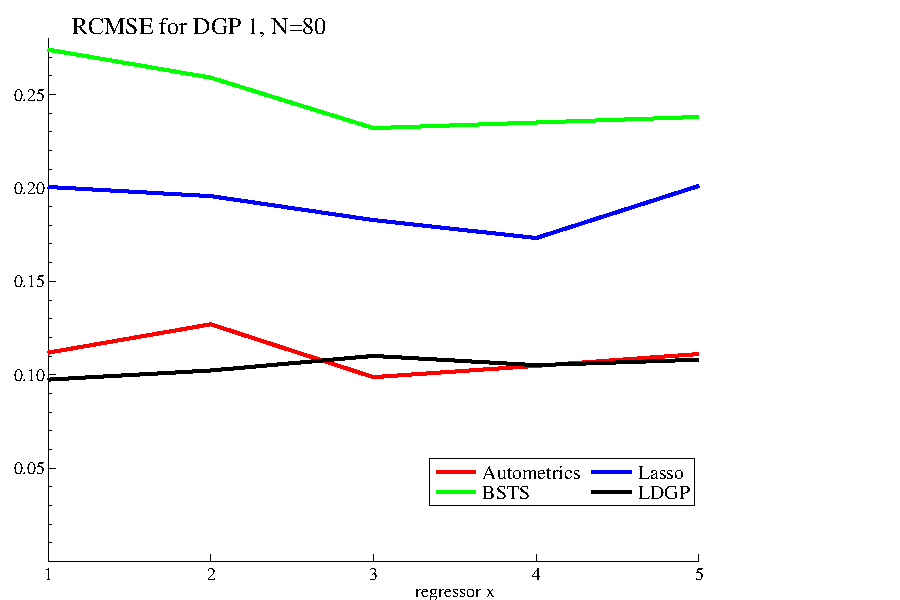
\includegraphics[scale=.5]{CMSE-DGP1a}
\caption{RCMSE for DGP 1}
\label{RCMSECase1a}
\end{minipage}%
\begin{minipage}{.5\textwidth}
\centering
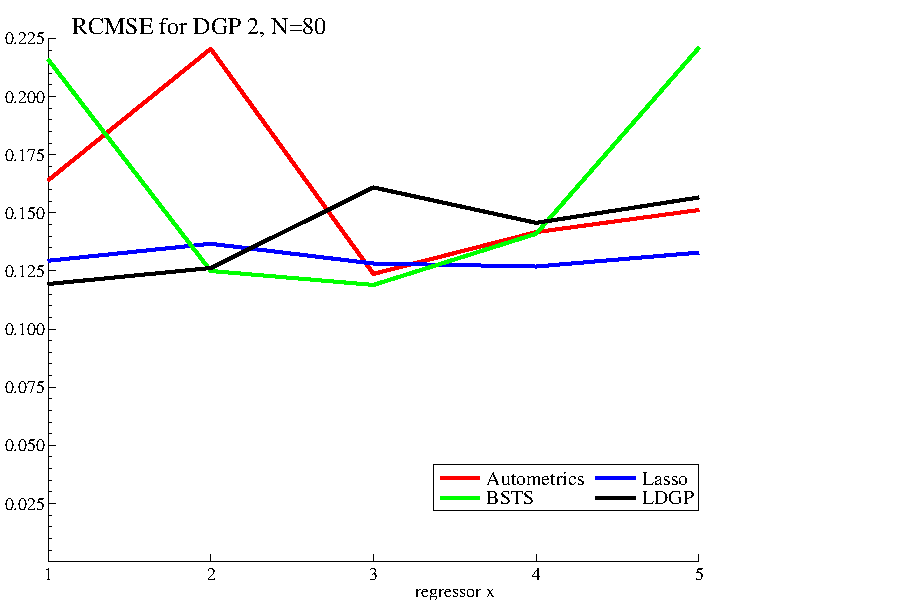
\includegraphics[scale=.5]{CMSE-DGP2a}
\caption{RCMSE for DGP 2}
\label{RCMSECase2a}
\end{minipage}

\end{figure}



\begin{figure}[h]

\begin{minipage}{.5\textwidth}
\centering
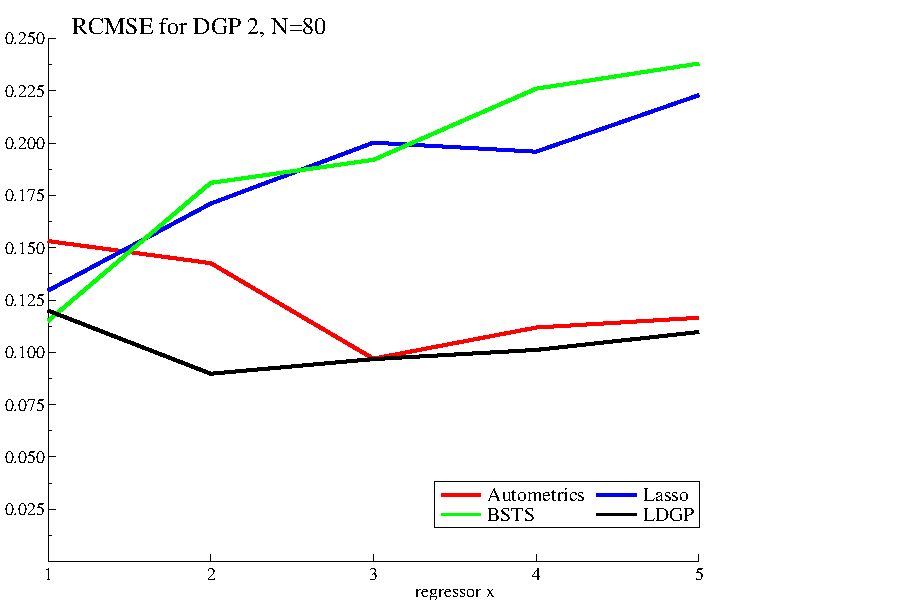
\includegraphics[scale=0.5]{CMSE-DGP3a}
\caption{RCMSE for DGP 3}
\label{fig:CMSEDGP3a}
\end{minipage}%
\begin{minipage}{.5\textwidth}
\centering
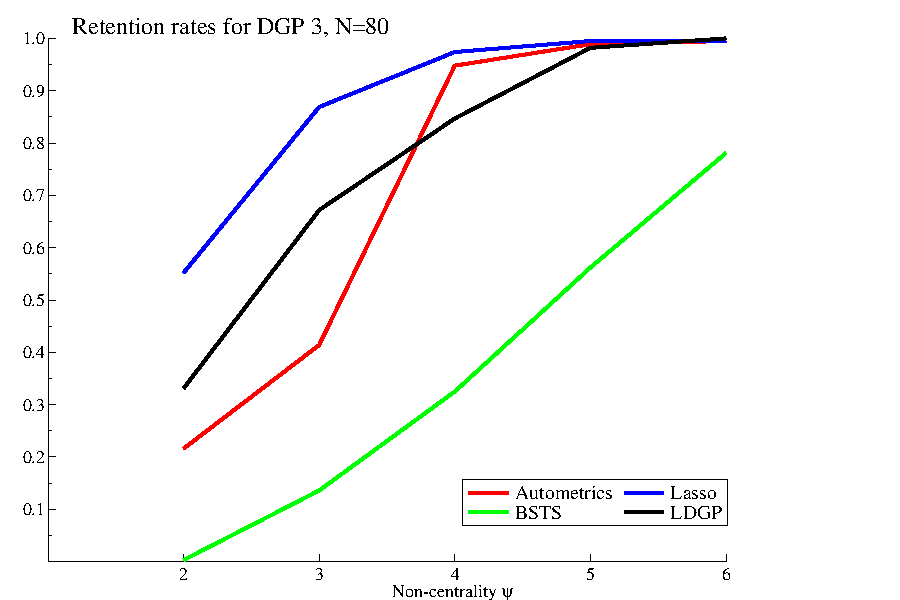
\includegraphics[scale=0.5]{RetRatesDGP3a}
\caption{Retention rates for DGP 3}
\label{fig:RetRatesDGP3a}

\end{minipage}

\end{figure}

\clearpage

The above results show the the Lasso consistently achieves the highest potency, and has the highest retention rates across all levels of $\psi$. Autometrics selects relevant regressors at a level which is generally similar to the theoretical retention probability (with a couple of exceptions) and does nearly as well as the Lasso when $\psi>4$. In comparison to Lasso and Autometrics, BSTS does not fair well when selecting relevant variables, even for variables with high values of $\psi$. Retention rates and potency measures do not change drastically between $N<T$ and $N>T$ when $\psi>4$, but results for lower values of $\psi$ vary quite significantly. 

BSTS consistently achieves the lowest gauge but its low potency and retention rates indicate that it tends to select very sparse models in general. The gauge for Lasso is generally very high and in the range of $0.12-0.22$, which along with the high levels of potency indicate that it selects models which include a lot of variables. In all of the six experiments, Autometrics has a gauge of close to the the significance level $\alpha = 0.01$, however in DGP2 with $\psi = 2$, the gauge is slightly higher at $0.029$. 

The RCMSE results are most easily interpreted by the graphs, which show that the results vary depending on values of $\psi$. As can be seen in Figures \ref{RCMSECase1a} and \ref{fig:CMSEDGP3a}, Autometrics performs well for high values of $\psi$. Figure \ref{fig:CMSEDGP3a} shows that Lasso and BSTS increasingly struggled as $\psi$ rises. Results are mixed in \ref{RCMSECase2a}, where there is a low non-centrality of $\psi=2$.

Both the Lasso and Autometrics have results similar to, or better than, the benchmark when examining the potency and retention rates. As mentioned, across the board, the Lasso has high potencies and low gauges, meaning that overall there is less 'selection' going on. It is a different story when examining the RCMSE results however; Autometrics is much closer to the benchmark (except in the case where $\psi=2$ where results are all over the place). This means the costs of inference are high in Lasso and BSTS.

The four biggest takeaways from this set of experiments are:
\begin{enumerate}
\item Autometrics consistently has a gauge close to the significance level and a retention rates/potencies close to the theoretical retention probabilities.
\item The Lasso scores high for successfully retaining irrelevant variables, but taken next to the gauges this is less impressive
\item BSTS selects models which are very sparse, which is seen clearly through its extremely low measures for gauge, and relatively low levels of potency.
\item The costs of inference vary with $\psi$, but generally are quite low with Autometrics, but high for both Lasso and BSTS.
\end{enumerate}





\clearpage

\subsection{Correlation between relevant regressors}

The second set of experiments considers several cases where there is correlation between the relevant regressors. There are two different DGPs considered, which again vary according to their coefficients $\gamma,\beta_{1},...,\beta_{5}$ and therefore their respective non-centralities. Note that $\beta_{1},...,\beta_{5}$ have been chosen so that the non-centralities in this set of experiments are inline with those in the first set of experiments, making the results more comparable. As in the first set of experiments, these two DGPs are nested in two different GUMs with $N=80$ and $N=120$. In all experiments, T=100. Thus, there are four separate experiments performed and reported on.   Let $\textbf{x}_{t}'=(x_{1,t},...,x_{N,t})$. The DGPs take the following form: 

$$y_{t}=\beta_{0} + \gamma y_{t-1}+\beta_{1}x_{1,t}+\beta_{2}x_{2,t}+ \beta_{3}x_{3,t}+ \beta_{4}x_{4,t}+ \beta_{5}x_{5,t} + \epsilon_{t}$$
$$\centerline{$\epsilon_{t} \sim $ IN[0,1] }$$
 $$\centerline{$\textbf{x}_{t} \sim $ IN\textsubscript{N}[0,$\Omega$]}$$

with $\omega_{kk} = 1 $, $\omega_{jk} = 0.9 $ for $j,k \leq 5$ and $\omega_{jk} = 0 $ elsewhere. Table \ref{DGPs4and5}  describes the two DGPs considered, from hereon referred to as DGP 4 and 5.

When the regressors are not orthogonal, as explained, simply using 1-cut selection on the LDGP is not a feasible baseline. The `best case scenario' in this case is then, is doing selection on the LDGP using the algorithms themselves. These results capture how effective the algorithm is in the case where the GUM includes exactly the correct regressors. The difference between the RCMSE from selection on the LDGP and selection from the GUM is therefore a measure of costs of inference. 

%For CMSE - no selection on LDGP is benchmark. 


%TABLE DGPs of experiments including orthogonal variables
\begin{table}[h]
\centering
\begin{tabular}{l|l|l|l|l|l|l|l}

& &$y_{t-1}$ &$x_{1}$ &$x_{2}$ &$x_{3}$ &  $x_{4}$ & $x_{5}$  \\
\hline
DGP 4 & $\beta$ & 0.5 & 0.58 &0.84 &1.25 &  1.55 & 1.75 \\

 	& $\psi$ & &2 &3 &4 &5 &6 \\
\hline
DGP 5 & $\beta$ & 0.5 & -0.58 &0.84 &-1.25 &  1.55 &-1.75 \\

 	& $\psi$ & &-2 &3 &-4 &5 &-6 \\

    
\end{tabular}
\caption{DGP specification for experiments with correlation between relevant regressors}
\label{DGPs4and5}
\end{table} 

Tables \ref{DGP4GP} and \ref{tDGP4RR} report the gauge, potency and retention rates for DGP4, and include results when selecting from the LDGP for each algorithm. Tables \ref{DGP5GP} and \ref{DGP5RetRates} do the same for DGP5. Tables \ref{DGP4CMSE} and \ref{LDGP5CMSE} report RCMSE results. Figures \ref{fig:RetRatesDGP4a}-\ref{fig:CMSEDGP5a} graph the results. Figures \ref{fig:CMSEDiffDGP4a} and \ref{fig:CMSEDiffDGP5a} graph the differences between RCMSE for each algorithm and their base line, and thus give an indication of the costs of inference for each of the algorithms.

% Table generated by Excel2LaTeX from sheet 'GPDGP4'
\begin{table}[htbp]
  \centering

    \begin{tabular}{rrrrr}

                   & \textbf{N=80} & \textbf{} & \textbf{N=120} & \textbf{} \\

          & \textbf{potency} & \textbf{gauge} & \textbf{potency} & \textbf{gauge} \\
    \textbf{Autometrics} & 0.777 & 0.014 & 0.769 & 0.013 \\
    \textit{from LDGP} & 0.797 &       & 0.797 &  \\
    \textbf{Lasso} & 0.993 & 0.108 & 0.993 & 0.077 \\
    \textit{from LDGP} & 0.994 &       & 0.994 &  \\
    \textbf{BSTS} & 0.690 & 0.000 & 0.677 & 0.000 \\
    \textit{from LDGP} & 0.784 &       & 0.784 &  \\

    \end{tabular}%
      \caption{Gauge and potency for DGP4}
  \label{DGP4GP}%
  
\end{table}%



     
% Table generated by Excel2LaTeX from sheet 'RetRatesChartDGP4'
\begin{table}[htbp]
  \centering

    \begin{tabular}{rrrrrrr}

          & \boldmath{}\textbf{$\psi$}\unboldmath{} & 2     & 3     & 4     & 5     & 6 \\

          & \boldmath{}\textbf{$p_{0.01}$}\unboldmath{}  & 0.266 & 0.645 & 0.914 & 0.990 & 0.999  \\
    \textbf{N=80} & \textbf{Autometrics} & 0.333 & 0.568 & 0.988 & 0.998 & 0.998 \\
    \textbf{} & \textbf{Lasso} & 0.977 & 0.990 & 1.000 & 1.000 & 1.000 \\
    \textbf{} & \textbf{BSTS} & 0.179 & 0.340 & 0.949 & 0.993 & 0.991 \\
    \textbf{N=120} & \textbf{Autometrics} & 0.316 & 0.611 & 0.923 & 0.996 & 0.999 \\
    \textbf{} & \textbf{Lasso} & 0.968 & 0.998 & 1.000 & 1.000 & 1.000 \\
    \textbf{} & \textbf{BSTS} & 0.155 & 0.369 & 0.874 & 0.988 & 0.999 \\
    \textbf{From LDGP} & \textbf{Autometrics} & 0.330 & 0.723 & 0.934 & 0.996 & 1.000 \\
          & \textbf{Lasso} & 0.979 & 0.993 & 1.000 & 1.000 & 1.000 \\
          & \textbf{BSTS} & 0.344 & 0.589 & 0.990 & 0.999 & 0.998 \\

    \end{tabular}%
      \caption{Retention rates for DGP4, including from LDGP}
  \label{tDGP4RR}%
\end{table}%


% Table generated by Excel2LaTeX from sheet 'GPDGP5'
\begin{table}[htbp]
  \centering

    \begin{tabular}{rrrrr}

          & \textbf{N=80} & \textbf{} & \textbf{N=120} & \textbf{} \\

          & \textbf{potency} & \textbf{gauge} & \textbf{potency} & \textbf{gauge} \\
    \textbf{Autometrics} & 0.716 & 0.014 & 0.719 & 0.014 \\
    \textit{from LDGP} & 0.775 &       & 0.775 &  \\
    \textbf{Lasso} & 0.429 & 0.088 & 0.374 & 0.057 \\
    \textit{from LDGP} & 0.986 &       & 0.986 &  \\
    \textbf{BSTS} & 0.531 & 0.000   & 0.439 & 0.000 \\
    \textit{from LDGP} & 0.675 &       & 0.675 &  \\

    \end{tabular}%
      \caption{Gauge and potency for DGP5}
  \label{DGP5GP}%
\end{table}%






% Table generated by Excel2LaTeX from sheet 'RetRatesDGP5Chart'
\begin{table}[htbp]
  \centering

    \begin{tabular}{rrrrrrr}

          & \boldmath{}\textbf{$\psi$}\unboldmath{} & -2    & 3     & -4    & 5     & -6 \\

        & \boldmath{}\textbf{$p_{0.01}$}\unboldmath{}  & 0.266 & 0.645 & 0.914 & 0.990 & 0.999  \\
    \textbf{N=80} & \textbf{Autometrics} & 0.255 & 0.355 & 0.981 & 0.996 & 0.994 \\
    \textbf{} & \textbf{Lasso} & 0.065 & 0.013 & 0.984 & 0.095 & 0.988 \\
    \textbf{} & \textbf{BSTS} & 0.022 & 0.056 & 0.798 & 0.827 & 0.951 \\
    \textbf{N=120} & \textbf{Autometrics} & 0.290 & 0.482 & 0.841 & 0.984 & 1.000 \\
    \textbf{} & \textbf{Lasso} & 0.254 & 0.007 & 0.590 & 0.019 & 0.998 \\
    \textbf{} & \textbf{BSTS} & 0.054 & 0.061 & 0.353 & 0.727 & 0.999 \\
    \textbf{From LDGP} & \textbf{Autometrics} & 0.336 & 0.631 & 0.925 & 0.981 & 1.000 \\
          & \textbf{Lasso} & 0.967 & 0.963 & 1.000 & 1.000 & 1.000 \\
          & \textbf{BSTS} & 0.150 & 0.267 & 0.974 & 0.989 & 0.995 \\
 
    \end{tabular}%
      \caption{Retention Rates for DGP5, including from LDGP}
  \label{DGP5RetRates}%
\end{table}%



% Table generated by Excel2LaTeX from sheet 'CMSEChartDGP4'
\begin{table}[htbp]
  \centering

    \begin{tabular}{rrrrrrrr}

          &       & $y_{t-1}$ & $x_{1}$ & $x_{2}$ & $x_{3}$ & $x_{4}$ & $x_{5}$ \\

          & $\beta$ &   0.5 & 0.58 &0.84 &1.25 &  1.55 & 1.75  \\
    \textbf{N=80} & \textbf{Autometrics} & 0.017 & 0.438 & 0.423 & 0.277 & 0.377 & 0.377 \\
    \textbf{} & \textbf{Lasso} & 0.038 & 0.279 & 0.339 & 0.259 & 0.292 & 0.307 \\
    \textbf{} & \textbf{BSTS} & 0.024 & 0.441 & 0.572 & 0.448 & 0.624 & 0.541 \\
    \textbf{N=120} & \textbf{Autometrics} & 0.016 & 0.432 & 0.332 & 0.431 & 0.405 & 0.342 \\
    \textbf{} & \textbf{Lasso} & 0.038 & 0.272 & 0.314 & 0.333 & 0.313 & 0.354 \\
    \textbf{} & \textbf{BSTS} & 0.020 & 0.530 & 0.555 & 0.606 & 0.626 & 0.499 \\
    \textbf{From LDGP} & \textbf{Autometrics} & 0.016 & 0.442 & 0.317 & 0.366 & 0.364 & 0.326 \\
          & \textbf{Lasso} & 0.021 & 0.266 & 0.329 & 0.255 & 0.286 & 0.297 \\
          & \textbf{BSTS} & 0.026 & 0.395 & 0.504 & 0.375 & 0.484 & 0.432 \\

    \end{tabular}%
      \caption{CMSE for DGP4, including baseline}
  \label{DGP4CMSE}%
\end{table}%


% Table generated by Excel2LaTeX from sheet 'CMSEDGP5Chart'
\begin{table}[htbp]
  \centering

    \begin{tabular}{rrrrrrrrr}

          &       & $y_{t-1}$ & $x_{1}$ & $x_{2}$ & $x_{3}$ & $x_{4}$ & $x_{5}$ &  \\

         & $\beta$ &   0.5 & -0.58 &0.84 &-1.25 &  1.55 & -1.75  \\
    \textbf{N=80} & \textbf{Autometrics} & 0.334 & 0.281 & 0.316 & 0.287 & 0.325 & 0.258 &  \\
    \textbf{} & \textbf{Lasso} & 0.120 & 0.463 & 0.656 & 0.778 & 1.074 & 1.225 &  \\
    \textbf{} & \textbf{BSTS} & 0.078 & 0.288 & 0.527 & 0.446 & 0.572 & 0.571 &  \\
    \textbf{N=120} & \textbf{Autometrics} & 0.273 & 0.292 & 0.303 & 0.296 & 0.341 & 0.257 &  \\
    \textbf{} & \textbf{Lasso} & 0.226 & 0.424 & 0.554 & 1.030 & 1.029 & 0.955 &  \\
    \textbf{} & \textbf{BSTS} & 0.097 & 0.405 & 0.510 & 0.603 & 0.722 & 0.496 &  \\
    \textbf{From LDGP} & \textbf{Autometrics} & 0.0514 & 0.342 & 0.239 & 0.330 & 0.334 & 0.330 &  \\
          & \textbf{Lasso} & 0.052 & 0.286 & 0.362 & 0.266 & 0.307 & 0.326 &  \\
          & \textbf{BSTS} & 0.071 & 0.342 & 0.482 & 0.384 & 0.411 & 0.408 &  \\

    \end{tabular}%
      \caption{CMSE for DGP5, including from LDGP}
  \label{LDGP5CMSE}%
\end{table}%






\begin{figure}[h]

\begin{minipage}{.5\textwidth}
\centering
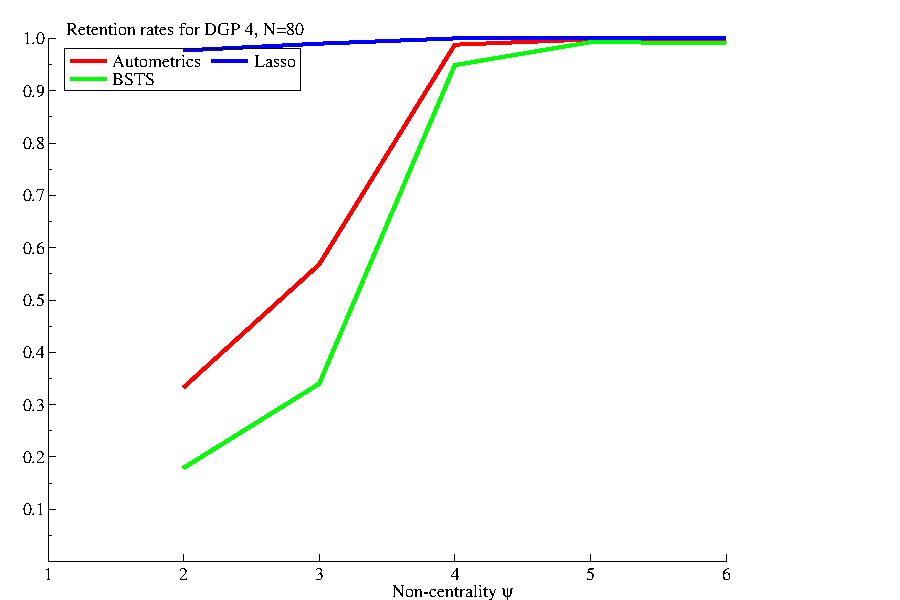
\includegraphics[scale=0.5]{RetRatesDGP4a}
\caption{Retention rates DGP 4 \newline N=80}
\label{fig:RetRatesDGP4a}
\end{minipage}%
\begin{minipage}{.5\textwidth}
\centering
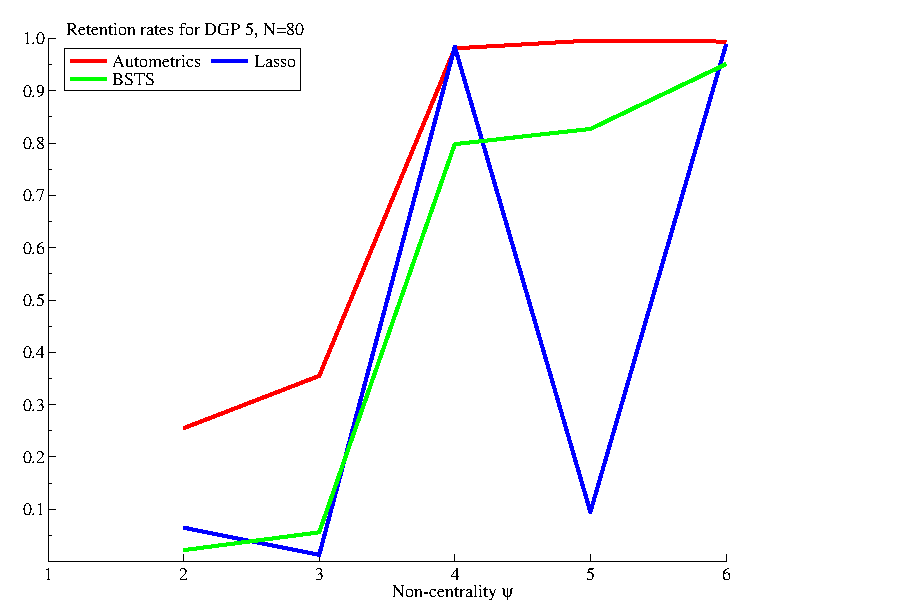
\includegraphics[scale=0.5]{RetRatesDGP5a}
\caption{Retention Rates DGP 5 \newline N=80}
\label{fig:RetRatesDGP5a}

\end{minipage}

\end{figure}









\begin{figure}[h]

\begin{minipage}{.5\textwidth}
\centering
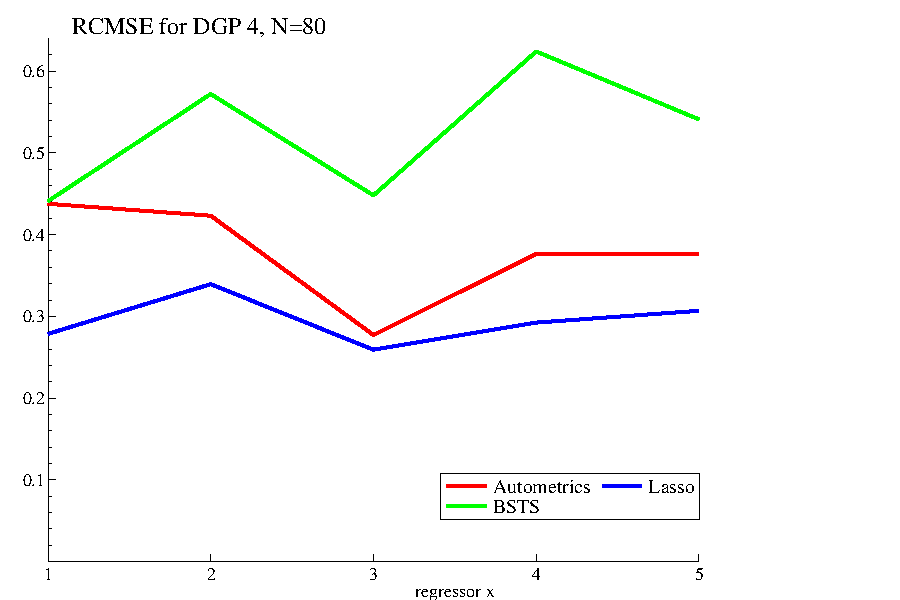
\includegraphics[scale=0.5]{CMSE-DGP4a}
\caption{CMSE for DGP 4 \newline N=80}
\label{fig:CMSEDGP4a}
\end{minipage}%
\begin{minipage}{.5\textwidth}
\centering
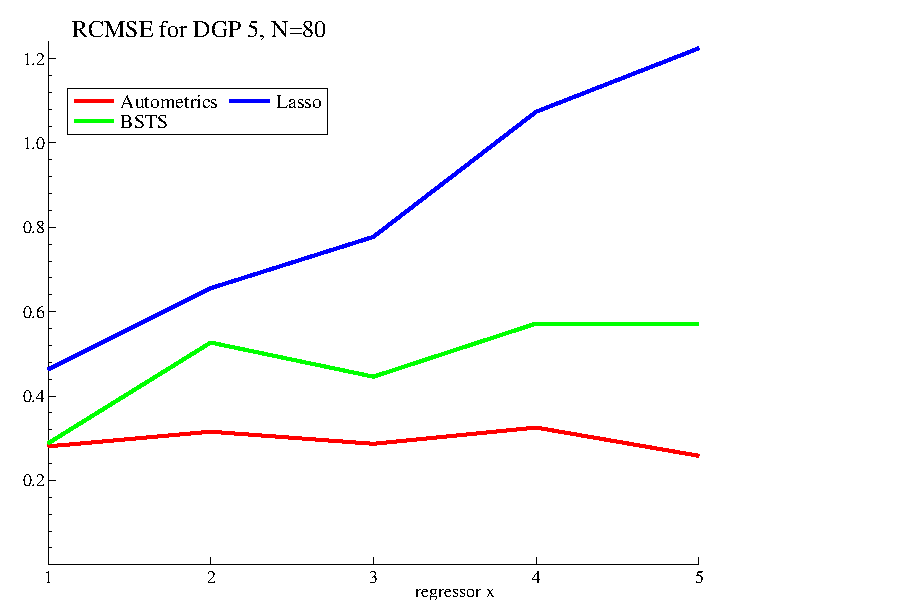
\includegraphics[scale=0.5]{CMSE-DGP5a}
\caption{CMSE for DGP 5 \newline N=80}
\label{fig:CMSEDGP5a}

\end{minipage}

\end{figure}

\begin{figure}[h]

\begin{minipage}{.5\textwidth}
\centering
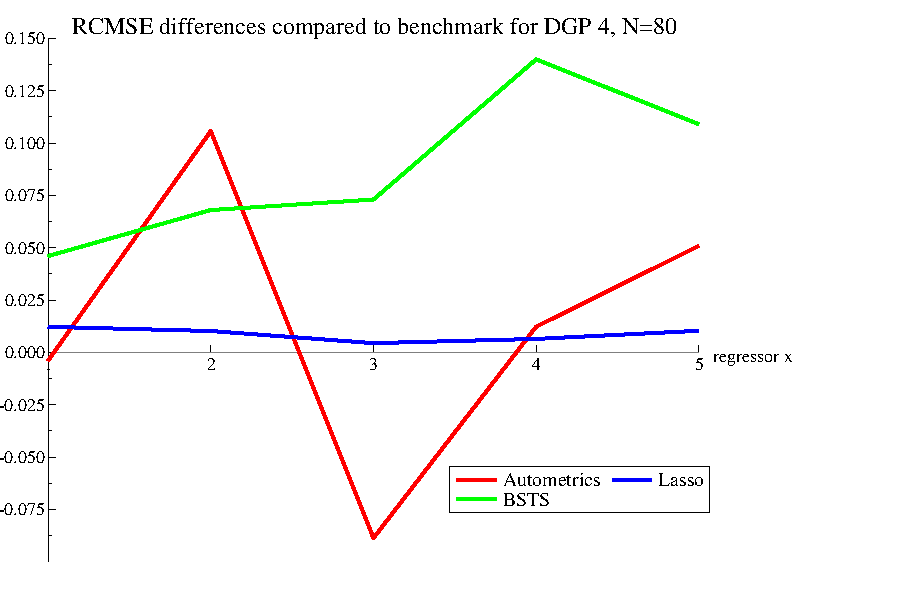
\includegraphics[scale=0.5]{CMSEDiffDGP4a}
\caption{CMSE Differences for DGP 4 \newline N=80}
\label{fig:CMSEDiffDGP4a}
\end{minipage}%
\begin{minipage}{.5\textwidth}
\centering
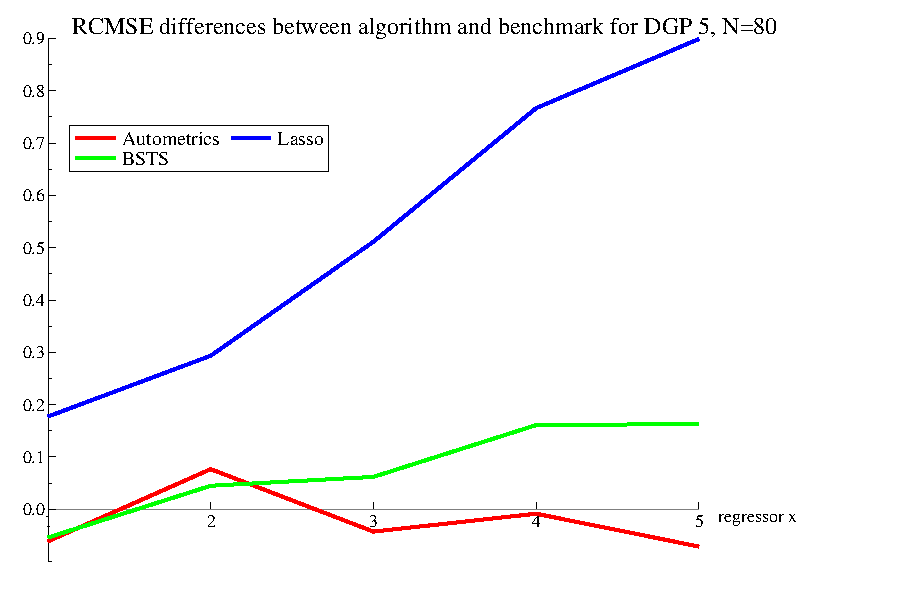
\includegraphics[scale=0.5]{CMSEDiffDGP5a}
\caption{CMSE Differences for DGP 5 \newline N=80}
\label{fig:CMSEDiffDGP5a}

\end{minipage}

\end{figure}





\clearpage

%Note that this section only examines results within the set of experiments where there is correlation between relevant regressors; analysis and comparison across the three sets of experiments will be discussed later on. 

First considering DGP4 results independently, when $\psi_{k} > 0, \forall k$, the Lasso has both the highest measures of potency and gauge. BSTS has the lowest gauge and Autometric's gauge is close to the significance level $\alpha$. Going from $N<T$ to $N>T$ in most cases does not have a big impact on the results. Both Autometrics and the Lasso have retention rates similar to their benchmark, while the benchmark for BSTS gives quite different results. The graph for the RCMSE differences is interesting (is there a meaningful way to interpret?), and shows there are almost no costs of search for Lasso, and for Autometrics there are in fact negative costs of search (meaning that sometimes parameter estimates are even more accurate than in the theoretical best case scenario).

Next looking at DGP5, it is clear that the algorithms struggle to varying degrees with alternating signs. This is particularly true for Lasso, with retention rates on regressors with $\psi>0$ being very low, irrespective of their magnitude. The search costs of Lasso also increase with $\psi$. The story for the gauge is similar to previous experiments; the gauge for BSTS is low in every experiment, the gauge for Autometrics is slightly higher than the significance level $\alpha$, and the gauge for Lasso varies across the experiments. The costs of search for both Autometrics and BSTS, as measured by the RCMSE differences, are quite low. 

Comparing the results from DGP4 to DGP5 gets interesting. While intuitively and theoretically the DGPs have nearly identical properties, the actual results vary drastically. Thinking about non-centrality as the signal-to-noise ratio, whether a variable has a positive or negative non-centrality should not impact how often it is selected by an algorithm; it is the magnitude of the the signal-to-noise ratio, $|\psi_{k}|$, which should influence an algorithm's ability to select that variable. Indeed, in the case of orthogonal variables, alternating signs did not result in potency and retention rate measures which were notably different from cases where the signs were all the same. 

It is immediately clear, however, that something strange is going on in DGP5 with alternative signs. DGP4 has retention rates which are as expected, increasing with $\psi$. In DGP5 while both Autometrics and BSTS have higher retention rates as $|\psi_{k}|$ rises, Lasso struggles to select either of the regressors with $\psi_{k}>0$. It should also be noted that while the retention rates do increase with $|\psi|$ for Autometrics and BSTS, the increase is not at all "uniform" and both Autometrics and BSTS are more successful at selecting variables with $|\psi|<0$. The RCMSE results illustrate the parameter estimates also vary across the DGPs. In DGP4, the Lasso has the lowest RCMSE for all variables, while it has the highest RCMSEs for all variables in DGP5. Furthermore, the RCMSEs increase with $\psi$ for the Lasso with alternating signs. 

The biggest takeaways from this second set of experiments are:

\begin{enumerate}
\item Selection when signs alternate produces remarkably different results (especially for Lasso)
\item When $\psi_{k} > 0 \ \forall \ k$ the Lasso selects a lot of both relevant and irrelevant variables, BSTS does not select many of either, and Autometrics is somewhere in the middle
\item
\item


\end{enumerate}



\subsection{Correlation between all regressors}


The third set of experiments considers several cases where there is correlation between all of the relevant regressors. There are two different DGPs considered, which again vary according to the coefficients $\gamma,\beta_{1},...,\beta_{5}$ and therefore their respective non-centralities. These two DGPs are nested, as previously, in two different GUMs with $N=80$ and $N=120$. In all experiments, T=100. There are four separate experiments performed and reported on. Let $\textbf{x}_{t}'=(x_{1,t},...,x_{N,t})$. The DGPs take the following form: 

$$y_{t}=\beta_{0} + \gamma y_{t-1}+\beta_{1}x_{1,t}+\beta_{2}x_{2,t}+ \beta_{3}x_{3,t}+ \beta_{4}x_{4,t}+ \beta_{5}x_{5,t} + \epsilon_{t}$$
$$\centerline{$\epsilon_{t} \sim $ IN[0,1] }$$
 $$\centerline{$\textbf{x}_{t} \sim $ IN\textsubscript{N}[0,$\Omega$]}$$

with $\omega_{kk} = 1 $, $\omega_{jk} = 0.8 $. The following table describes the two DGPs considered, from hereon referred to as DGP 6 and 7:


%TABLE DGPs of experiments including orthogonal variables
\begin{table}[h]


\label{my-label}
\centering
\begin{tabular}{l|l|l|l|l|l|l|l}

& &$y_{t-1}$ &$x_{1}$ &$x_{2}$ &$x_{3}$ &  $x_{4}$ & $x_{5}$  \\
\hline
DGP 6 & $\beta$ & 0.5 & 0.4&0.6 &0.9&1.1  &1.25  \\

 	& $\psi$ & &2 &3 &4 &5 &6 \\
\hline
DGP 7 & $\beta$ & 0.5 & -0.4&0.6 &-0.9&1.1  &-1.25 \\

 	& $\psi$ & &-2 &3 &-4 &5 &-6 \\

    
\end{tabular}
\caption{DGP specification for experiments with correlation between all regressors}
\end{table} 


The following tables report the potency, gauge, retention rates and RCMSE for DGP 6 and DGP 7. The results are also graphed. 

% Table generated by Excel2LaTeX from sheet 'DGP6GP'
\begin{table}[htbp]
  \centering

    \begin{tabular}{rrrrr}

          & \textbf{N=80} & \textbf{} & \textbf{N=120} & \textbf{} \\

          & \textbf{potency} & \textbf{gauge} & \textbf{potency} & \textbf{gauge} \\
    \textbf{Autometrics} & 0.736 & 0.016 & 0.718 & 0.015 \\
    \textit{from LDGP} & 0.798 &       & 0.798 &  \\
    \textbf{Lasso} & 0.909 & 0.182 & 0.894 & 0.131 \\
    \textit{from LDGP} & 0.993 &       & 0.993 &  \\
    \textbf{BSTS} & 0.653 & 0.004 & 0.631 & 0.005 \\
    \textit{from LDGP} & 0.764 &       & 0.764 &  \\

    \end{tabular}%
      \caption{Gauge and potency for DGP6}
  \label{DGP6GP}%
\end{table}%




% Table generated by Excel2LaTeX from sheet 'RetRatesDGP6Chart'
\begin{table}[htbp]
  \centering

    \begin{tabular}{rrrrrrr}

          & \boldmath{}\textbf{$\psi$}\unboldmath{} & 2    & 3     & 4    & 5     & 6 \\

          & \textbf{$p_{0.01}$}\unboldmath{}  & 0.266 & 0.645 & 0.914 & 0.990 & 0.999  \\
    \textbf{N=80} & \textbf{Autometrics} & 0.262 & 0.439 & 0.985 & 0.996 & 0.996 \\
    \textbf{} & \textbf{Lasso} & 0.766 & 0.778 & 1.000 & 1.000 & 1.000 \\
    \textbf{} & \textbf{BSTS} & 0.116 & 0.251 & 0.923 & 0.984 & 0.990 \\
    \textbf{N=120} & \textbf{Autometrics} & 0.212 & 0.524 & 0.890 & 0.966 & 0.999 \\
    \textbf{} & \textbf{Lasso} & 0.560 & 0.924 & 0.991 & 0.998 & 0.999 \\
    \textbf{} & \textbf{BSTS} & 0.093 & 0.285 & 0.810 & 0.971 & 0.997 \\
    \textbf{From LDGP} & \textbf{Autometrics} & 0.327 & 0.729 & 0.938 & 0.995 & 1.000 \\
          & \textbf{Lasso} & 0.969 & 0.994 & 1.000 & 1.000 & 1.000 \\
          & \textbf{BSTS} & 0.281 & 0.554 & 0.990 & 0.998 & 0.999 \\

    \end{tabular}%
      \caption{Retention Rates for DGP6}
  \label{DGP6RetRates}%
\end{table}%

% Table generated by Excel2LaTeX from sheet 'CMSEDGP6Chart'
\begin{table}[htbp]
  \centering

    \begin{tabular}{rrrrrrrr}
  
          &       & $y_{t-1}$ & $x_{1}$ & $x_{2}$ & $x_{3}$ & $x_{4}$ & $x_{5}$ \\

          &       & 0.5 & 0.4&0.6 &0.9&1.1  &1.25  \\
    \textbf{N=80} & \textbf{Autometrics} & 0.025 & 0.318 & 0.313 & 0.190 & 0.241 & 0.250 \\
    \textbf{} & \textbf{Lasso} & 0.041 & 0.230 & 0.347 & 0.257 & 0.349 & 0.315 \\
    \textbf{} & \textbf{BSTS} & 0.036 & 0.318 & 0.404 & 0.386 & 0.386 & 0.348 \\
    \textbf{N=120} & \textbf{Autometrics} & 0.023 & 0.329 & 0.227 & 0.263 & 0.254 & 0.232 \\
    \textbf{} & \textbf{Lasso} & 0.033 & 0.254 & 0.313 & 0.376 & 0.462 & 0.389 \\
    \textbf{} & \textbf{BSTS} & 0.026 & 0.306 & 0.370 & 0.430 & 0.428 & 0.346 \\
    \textbf{From LDGP} & \textbf{Autometrics} & 0.024022 & 0.30655 & 0.21898 & 0.259 & 0.255 & 0.230 \\
          & \textbf{Lasso} & 0.029 & 0.192 & 0.234 & 0.182 & 0.204 & 0.211\\
          & \textbf{BSTS} & 0.036 & 0.275 & 0.361 & 0.258 & 0.337 & 0.314 \\
 
    \end{tabular}%
      \caption{CMSE for DGP6}
  \label{DGP6CMSE}%
\end{table}%


% Table generated by Excel2LaTeX from sheet 'GPDGP7'
\begin{table}[htbp]
  \centering
 
    \begin{tabular}{rrrrr}

          & \textbf{N=80} & \textbf{} & \textbf{N=120} & \textbf{} \\

          & \textbf{potency} & \textbf{gauge} & \textbf{potency} & \textbf{gauge} \\
    \textbf{Autometrics} & 0.718 & 0.014 & 0.707 & 0.014 \\
    \textit{from LDGP} & 0.778 & N/A   & 0.778 & N/A \\
    \textbf{Lasso} & 0.787 & 0.154 & 0.823 & 0.131 \\
    \textit{from LDGP} & 0.986 & N/A   & 0.986 & N/A \\
    \textbf{BSTS} & 0.512 & 0.001 & 0.401 & 0.001 \\
    \textit{from LDGP} & 0.6572 & N/A   & -0.6572 & N/A \\

    \end{tabular}%
     \caption{Gauge and potency for DGP7}
  \label{DGP7GP}%
\end{table}%


% Table generated by Excel2LaTeX from sheet 'RetRatesDGP7Chart'
\begin{table}[htbp]
  \centering

    \begin{tabular}{rrrrrrr}

          & \boldmath{}\textbf{$\psi$}\unboldmath{} & -2    & 3     & -4    & 5     & -6 \\

          & \textbf{$p_{0.01}$}\unboldmath{}  & 0.266 & 0.645 & 0.914 & 0.990 & 0.999  \\
    \textbf{N=80} & \textbf{Autometrics} & 0.230 & 0.380 & 0.988 & 0.993 & 0.998 \\
    \textbf{} & \textbf{Lasso} & 0.507 & 0.466 & 0.999 & 0.963 & 1.000 \\
    \textbf{} & \textbf{BSTS} & 0.011 & 0.041 & 0.812 & 0.791 & 0.907 \\
    \textbf{N=120} & \textbf{Autometrics} & 0.253 & 0.510 & 0.803 & 0.972 & 0.999 \\
    \textbf{} & \textbf{Lasso} & 0.603 & 0.683 & 0.904 & 0.926 & 1.000 \\
    \textbf{} & \textbf{BSTS} & 0.037 & 0.051 & 0.303 & 0.641 & 0.971 \\
    \textbf{From LDGP} & \textbf{Autometrics} & 0.330 & 0.649 & 0.931 & 0.980 & 1.000 \\
          & \textbf{Lasso} & 0.964 & 0.967 & 1.000 & 1.000 & 1.000 \\
          & \textbf{BSTS} & 0.103 & 0.242 & 0.965 & 0.983 & 0.993 \\

    \end{tabular}%
     \caption{Retention Rates for DGP7}
  \label{DGP7RetRates}%
\end{table}%

% Table generated by Excel2LaTeX from sheet 'CMSEDGP7Chart'
\begin{table}[htbp]
  \centering

    \begin{tabular}{rrrrrrrr}

          &       & $y_{t-1}$ & $x_{1}$ & $x_{2}$ & $x_{3}$ & $x_{4}$ & $x_{5}$ \\

     &     & 0.5 & -0.4&0.6 &-0.9&1.1  &-1.25  \\
    \textbf{N=80} & \textbf{Autometrics} & 0.059 & 0.286 & 0.267 & 0.187 & 0.224 & 0.246 \\
    \textbf{} & \textbf{Lasso} & 0.078 & 0.257 & 0.415 & 0.330 & 0.514 & 0.532 \\
    \textbf{} & \textbf{BSTS} & 0.111 & 0.188 & 0.358 & 0.327 & 0.405 & 0.438 \\
    \textbf{N=120} & \textbf{Autometrics} & 0.070 & 0.328 & 0.230 & 0.221 & 0.253 & 0.232 \\
    \textbf{} & \textbf{Lasso} & 0.121 & 0.257 & 0.370 & 0.526 & 0.564 & 0.421 \\
    \textbf{} & \textbf{BSTS} & 0.147 & 0.272 & 0.362 & 0.458 & 0.515 & 0.359 \\
    \textbf{From LDGP} & \textbf{Autometrics} & 0.059 & 0.246 & 0.168 & 0.237 & 0.236 & 0.232 \\
          & \textbf{Lasso} & 0.059 & 0.205 & 0.256 & 0.190 & 0.216 & 0.229 \\
          & \textbf{BSTS} & 0.084 & 0.236 & 0.344 & 0.281 & 0.294 & 0.298 \\

    \end{tabular}%
      \caption{CMSE for DGP7}
  \label{DGP7CMSE}%
\end{table}%













\begin{figure}[h]

\begin{minipage}{.5\textwidth}
\centering
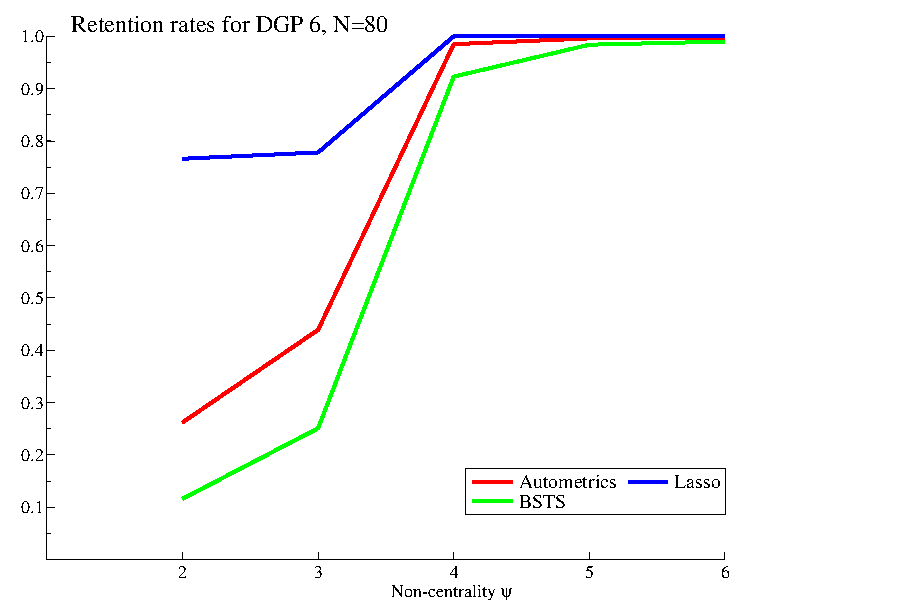
\includegraphics[scale=0.5]{RetRatesDGP6a}
\caption{Retention rates DGP 6 \newline N=80}
\label{fig:RetRatesDGP6a}
\end{minipage}%
\begin{minipage}{.5\textwidth}
\centering
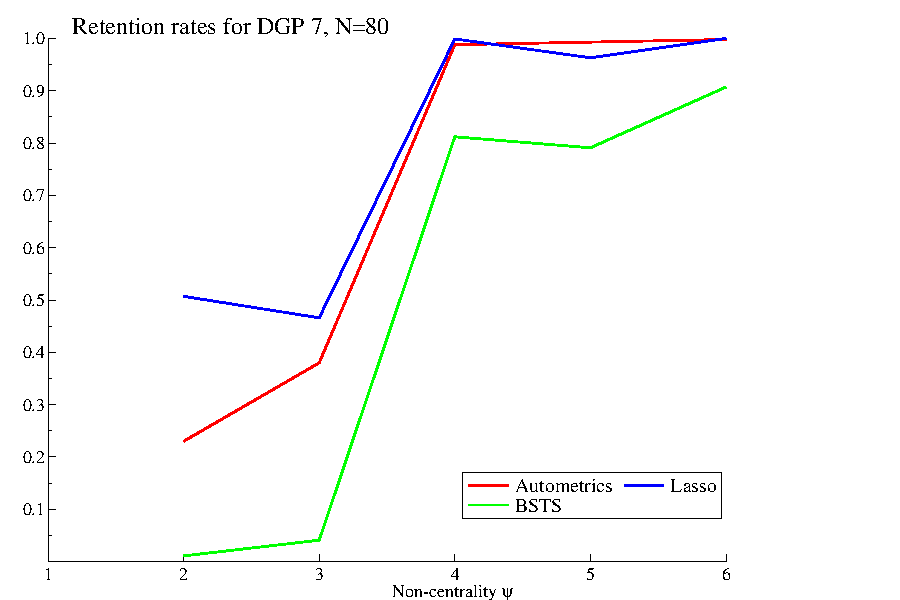
\includegraphics[scale=0.5]{RetRatesDGP7a}
\caption{Retention Rates DGP 7 \newline N=80}
\label{fig:RetRatesDGP7a}

\end{minipage}

\end{figure}

\begin{figure}[h]

\begin{minipage}{.5\textwidth}
\centering
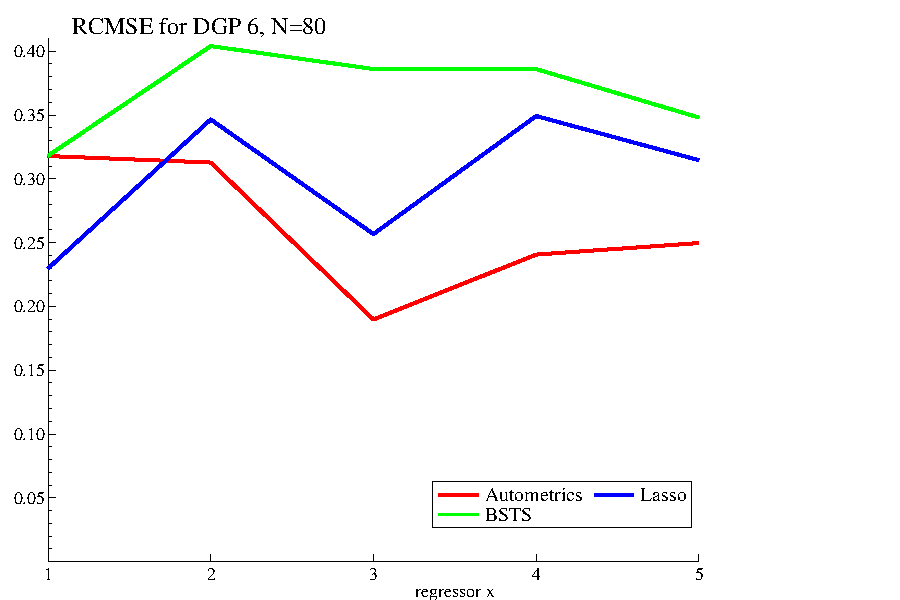
\includegraphics[scale=0.5]{RCMSE-DGP6a}
\caption{CMSE DGP 6 \newline N=80}
\label{fig:CMSEDGP6a}
\end{minipage}%
\begin{minipage}{.5\textwidth}
\centering
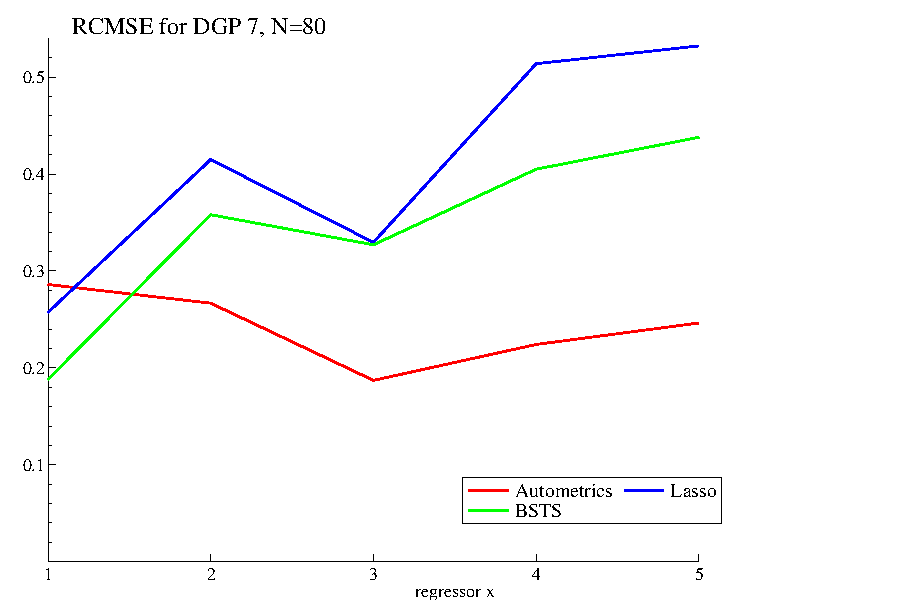
\includegraphics[scale=0.5]{RCMSE-DGP7a}
\caption{CMSE DGP 7 \newline N=80}
\label{fig:CMSEDGP7a}

\end{minipage}

\end{figure}




\begin{figure}[h]

\begin{minipage}{.5\textwidth}
\centering
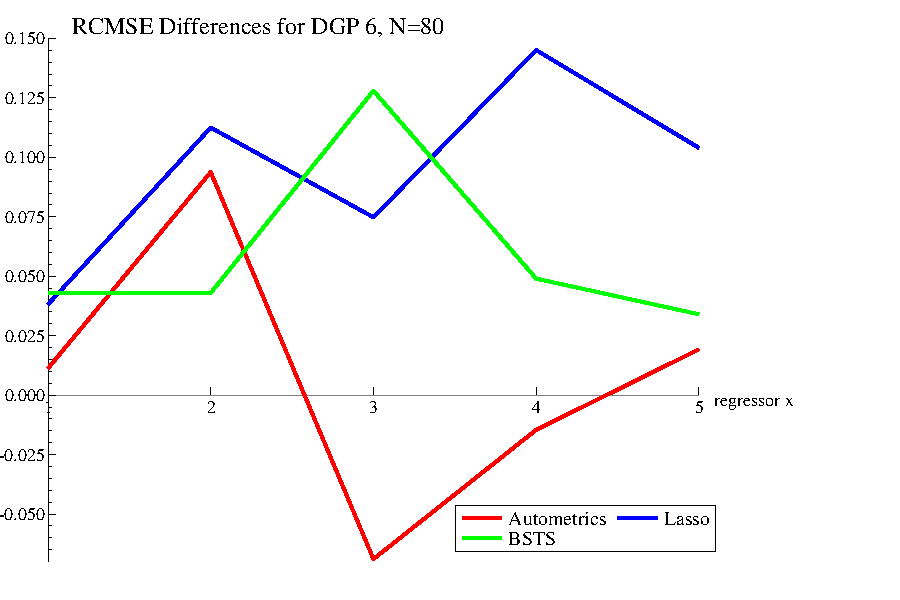
\includegraphics[scale=0.5]{RCMSEDiffDGP6a}
\caption{CMSE DGP 6 \newline N=80}
\label{fig:CMSEDGP6a}
\end{minipage}%
\begin{minipage}{.5\textwidth}
\centering
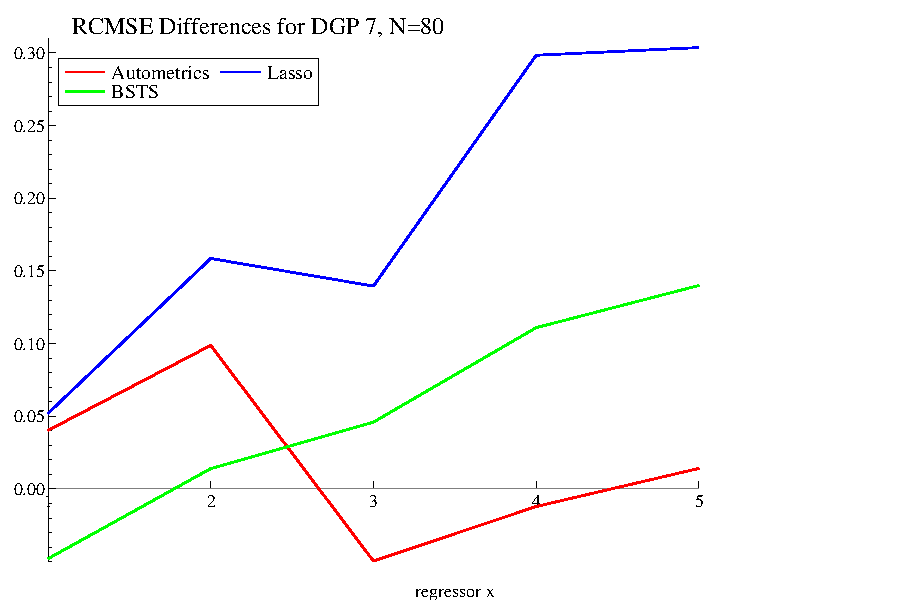
\includegraphics[scale=0.5]{RCMSEDiffDGP7a}
\caption{CMSE DGP 7 \newline N=80}
\label{fig:CMSEDGP7a}

\end{minipage}

\end{figure}

\clearpage

First looking at the results from DGP6, the Lasso is quite effective at identifying relevant variables. It also tends to select many irrelevant variables overall, as evidenced by the high gauge. When $\psi>3$, the retention rates for all three algorithms are very high. The gauge for Autometrics is slightly higher than the significance level $\alpha$, and almost 0 for BSTS. The RCMSE are generally highest for BSTS and lowest for Autometrics. Search costs are lowest for Autometrics. 

Turning to the DGP7 results, the retention rates are similar to those of DGP 6 but different in a subtle but important way. Both Lasso and BSTS struggle to pick up variables with $\psi_{k}>0$. Similarly, Lasso struggles to estimate the parameters on variables with $\psi_{k}>0$. These difficulties are not as pronounced as in the previous set of experiments, but clear nonetheless. While Lasso and BSTS struggle increasingly to estimate the parameter estimates as $|\psi|$ increases, Autometrics has RCMSEs which are low and consistent for all variables. 

Comparing DGP6 and DGP7, several important differences arise. While in theory the DGPs are very similar with almost identical properties, the results vary. Lasso and BSTS again seem to to struggled with alternating signs, both in terms of how effectively they pick up relevant variables, and how accurate the parameter estimates are. The measures of gauge are consistent across all algorithms in both DGP6 and DGP7; again BSTS with the lowest gauge near 0, Lasso with the highest in the range of 0.13-0.18, and Autometrics in the middle with gauges slightly above the significance level.

The takeaways from this set of experiments are:
\begin{enumerate}
\item Alternating signs matters a lot of Lasso, a reasonable amount for BSTS and a little for Autometrics
\item Lasso is excellent at selecting relevant variables when all the signs are the same, but not very good at excluding irrelevant variables
\item The gauge for Autometrics is very consistently slightly above the significance level for all experiments 
\item BSTS generally selects very sparse models, which do not include many relevant or irrelevant variables 
\end{enumerate} 

\clearpage
























 








\newpage

\section{Results Summary}

Evaluating the algorithms up until this point has focused on comparing the results from model selection conditional on a known correlation structure between the regressors. Therefore, when thinking about what the results in the previous section say about empirical model selection, the correlation structure of the variables under consideration must be taken into account. For example, if a researcher used Autometrics or Lasso on a set of orthogonal variables, she would know that the model selected by Autometrics included $\alpha$ percent of the irrelevant variables, and the model selected by Lasso included 15-20 percent of the irrelevant variables. Similarly, she would know there was a 99 percent change that a variable with a signal-to-noise ratio of 4 was included in the selected model. This statements rely on orthogonality, however. Given that the world is dynamic, full of relationships and extremely interdependent, orthogonal results on their own are of limited use. Because a researcher never knows the true DGP, she cannot possibly know what the true correlation structure is. Thus, to truly be able to interpret and say something meaningful about the effectiveness of model selection empirically, it is vital to understand how different `settings' or correlation structures produce different results. Since a researcher can never know the true DGP and and therefore can not qualify results in this manner, ideally model selection results should not depend on what the correlation structure is.

A desirable property of model selection would be for a variable with a given `signficance', which can be measured by its non-centrality, to be selected at the same level regardless of the properties of the other variables in the GUM. It is for this reason that in each of the three sets of experiments, $\beta_{1},...,\beta_{5}$ were chosen so that non-centralities are the same and retention rates and RCMSEs are comparable across experiments. Looking at how results vary across the three different correlation structures is a therefore a straightforward way to analyze how orthogonality or otherwise influences results across values of $\psi$. Table \ref{tab:SummaryPositive} shows a summary of the results for DGP3, DGP4, and DGP6 for N=80. Similarly, Table \ref{tab:SummaryAlt} shows the results for DGPs with alternating signs. Note that results from alternating signs when the regressors are orthogonal are largely the same as when the signs are all the same, and were not reported earlier. 

% Table generated by Excel2LaTeX from sheet 'Allpositive-noformulas'

\begin{landscape}

\begin{table}[htbp]
  \centering

    \begin{tabular}{rrrrrrrrrr}
   & \multicolumn{3}{l}{Autometrics} & \multicolumn{3}{l}{Lasso} & \multicolumn{3}{l}{BSTS} \\
 
    $\psi$ & Orthogonal  & Some Corr & All Corr & Orthogonal  & Some Corr & All Corr & Orthogonal  & Some Corr & All Corr \\
    2     & 0.216 & 0.333 & 0.262 & 0.552 & 0.977 & 0.766 & 0.003 & 0.179 & 0.116 \\
    3     & 0.414 & 0.568 & 0.439 & 0.869 & 0.99  & 0.778 & 0.136 & 0.34  & 0.251 \\
    4     & 0.948 & 0.988 & 0.985 & 0.974 & 1     & 1     & 0.325 & 0.949 & 0.923 \\
    5     & 0.989 & 0.998 & 0.996 & 0.995 & 1     & 1     & 0.562 & 0.993 & 0.984 \\
    6     & 0.995 & 0.998 & 0.996 & 0.996 & 1     & 1     & 0.781 & 0.991 & 0.99 \\
   
    Potency & 0.712 & 0.777 & 0.736 & 0.877 & 0.993 & 0.909 & 0.361 & 0.690 & 0.653 \\
    Gauge & 0.018 & 0.014 & 0.016 & 0.179 & 0.108 & 0.182 & 0.001 & 0.000 & 0.004 \\


 
    \end{tabular}%
 
    \caption{Summary results for all positive $\psi$}
     \label{tab:SummaryPositive}%
\end{table}%

% Table generated by Excel2LaTeX from sheet 'Alternating-noformulas'
\begin{table}[htbp]
  \centering

    \begin{tabular}{rrrrrrrrrr}

          & \multicolumn{3}{l}{Autometrics} & \multicolumn{3}{l}{Lasso} & \multicolumn{3}{l}{BSTS} \\

    $\psi$ & Orthogonal & Some Corr & All Corr & Orthogonal & Some Corr & All Corr & Orthogonal  & Some Corr & All Corr \\
    -2    & 0.24  & 0.255 & 0.23  & 0.608 & 0.065 & 0.507 & 0.007 & 0.022 & 0.011 \\
    3     & 0.476 & 0.355 & 0.38  & 0.74  & 0.013 & 0.466 & 0.043 & 0.056 & 0.041 \\
    -4    & 0.928 & 0.981 & 0.988 & 0.981 & 0.984 & 0.999 & 0.349 & 0.798 & 0.812 \\
    5     & 0.993 & 0.996 & 0.993 & 1     & 0.095 & 0.963 & 0.943 & 0.827 & 0.791 \\
    -6    & 0.996 & 0.994 & 0.998 & 0.998 & 0.988 & 1     & 0.792 & 0.951 & 0.907 \\
    Potency & 0.727 & 0.716 & 0.718 & 0.865 & 0.429 & 0.787 & 0.427 & 0.531 & 0.512 \\
    Gauge & 0.018 & 0.014 & 0.014 & 0.176 & 0.088 & 0.154 & 0.000 & 0.000 & 0.001 \\

    \end{tabular}%
  
    \caption{Summary results for alternating $\psi$}
    \label{tab:SummaryAlt}%
\end{table}%

\end{landscape}

These two tables contain many interesting insights. The results for Autometrics do not vary significantly across the different correlation structures, both when $\psi_{k}>0,\forall k$ and when the signs of $\psi$ alternate. As $|\psi|$ increases, correlation matters less and results converge to 1. The gauge is also consistent across correlation structures, fluctuating between 0.014 and 0.018.  The Lasso, on the other hand, exhibits a very different story. While when $\psi_{k}>0, \forall k$, and $\psi>3$ the retention rates are consistent across the correlation structures, this is not the case when the signs are alternating. In fact, in the case of alternating signs, Lasso picks up variable k with $\psi_{k}=3$, 74\% of the time when the regressors are orthogonal, compared to 1\% of the time when there is correlation between the relevant regressors, and 46\% of the time when there is correlation between all regressors. The gauge in Lasso experiments is also remarkably varied, ranging between 0.09 and 0.18. These discrepancies and their implications are huge. The same is true, but to a lesser extent, for BSTS where there is notable variation in retention rates across the three correlation structures, especially when $|\psi|<4$. The gauge for BSTS, on the other hand, has almost no variation.

Figure \ref{fig:GaugePot} provides an interesting visual representation of the results in the previous two tables. The potency and gauge are plotted against each other for both N=80 and N=120, meaning that a total of twelve experiments are graphed. The experiments graphed have properties such that one would expect MCMC results to be similar. The ideal algorithm would have all of its points bunched in the upper left corner of the graph. As can be easily seen, the Lasso and BSTS are decidedly not even in the upper left quadrant. In fact, Lasso has points all over the graph. While BSTS consistently achieves a low gauge, it fairs poorly when it comes to potency. Autometrics points, on the other hand, are grouped together closely. While it may not always have as high a potency as Lasso, or as low a gauge as BSTS, it does reasonably well in both and perhaps most importantly it is consistent in the sense that the correlation strucuture of the regressors has no bearing on the results. 

\begin{figure}[h]


\centering
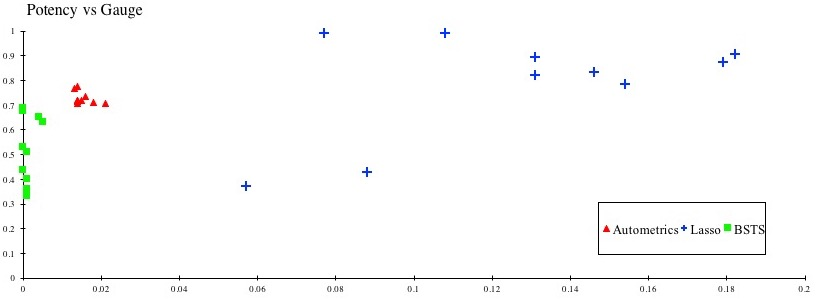
\includegraphics[scale=.5]{GPGraph}
\caption{Scatter plot of gauge vs. potency across all experiments}
\label{fig:GaugePot}


\end{figure}


\textbf{What do the MCMC mean for empirical model selection?}

As should be clear by now, model selection is difficult to evaluate empirically; it is impossible to judge how `good' a selected model is because it is impossible to know what to be judging against. This is why the results from MCMC simulations are so important and useful, and in particular why analyzing what happens when correlation structures change is vital. Because a modeler can never know what the properties of the relevant variables are, to draw valuable insight from selected models it is key that model selection not be reliant on what those properties are. With this in mind, the results in this study imply that a modeler performing model selection using the three algorithms can assume the following:

\textbf{Autometrics}
\begin{enumerate}
\item There are slightly higher than 100($\alpha$)\% of the total number of irrelevant variables included in the selected model. 
\item The probability that a variable with `significance', in signal-to-noise terms of $\psi$ has been selected can be approximated by the theoretical retention probability formula.
\item The costs of inference, or equivalently the parameter estimate accuracy, does not vary according to how `significant' a variable is. (Bias correction has not been employed here as discussed earlier, but studies show that this a cost-less way of improving parameter accuracy)
\item The costs of search for using Autometrics are minimal and sometimes even negative. That is, a researcher will `lose' almost nothing employing Autometrics, but stands to gain immensely.
\end{enumerate}

\textbf{Lasso}
\begin{enumerate}
\item There can be anywhere in the range of 8-20\% of the total number of irrelevant variables included in the selected model.
\item If all important variables in the model happen to be relevant to the dependent variables in the same `direction' (i.e. all have matter in either a positive or negative way for the dependent variable) , then Lasso will identify and select them with a high probability. In particular, a variable with a signal-to-noise ratio of $\psi>3$ has over a 97\% change of being selected.
\item The probability of selecting a relevant variable with a lower signal-to-noise ratio varies according to how correlated it is with the other variables in the model. For example the probability of selecting a variable with a signal-to-noise ratio of $\psi=2$ can be anywhere in the range of 55-98 percent. 
\item Parameter estimates become increasingly inaccurate the more `significant' a variable is.
\end{enumerate}

\textbf{BSTS}
\begin{enumerate}
\item There are almost no irrelevant variables (around 0.1 percent) included in the selected model.
\end{enumerate}






 

 

\chapter{An Application: Using Automatic Model Selection for Nowcasting}

In this section, automatic model selection is applied to the problem of nowcasting. It is important to note that while nowcasting may be a fruitful application of automatic model selection, nowcasting (or forecasting) is a fundamentally different problem with a different objective than model selection. This section is included to show an interesting application of the algorithms, and the results should be interpreted separately from the previous section. 

\section{Google Search Query Data}

The amount of information Google collects through search queries is difficult to comprehend. Every second, 40 000 Google searches are processed. That means there are over 3.5 billion Google searches each day and over 1 trillion Google searches per year. People turn to Google to get information on just about every aspect of their lives, so it makes sense that Google search queries contain large amounts of information about the state of the world. It is easy to think of cases where Google search queries many contain information about macroeconomic indicators. For example, if an individual loses their job, one of the first places they are likely to go is Google to determine how unemployment benefits are. Google is also one of the first places they would turn to being searching for a new job. Thus, Google search queries potentially tell a story about the current state of unemployment in the economy. Similarly, individuals looking to buy new cars are likely to turn to Google to research their options before actually going to a dealership. Google search queries related to new cars could therefore provide insight into current consumer sentiment. 

Google has recently developed several online tools, namely Google Trends and Google Correlate, which allow users to analyze what people have been Googling. Google Trends allows users to enter any search term and see the frequency with which it has been searched over time. Google Correlate allows users to enter a search query and see which other search queries are most correlated with it. Google Correlate has an additional feature which allows the user to enter their own time series and provides the user with the search queries which are most correlated with their submitted time series.

\subsection{Google Flu Trends}

One of the first ways in which the information contained in Google search query data was harnessed and put to use was with the Google Flu Trends application. The Center for Disease Control (CDC) in America publishes statistics on the proportion of doctor or hospital visits due to influenza like illness symptoms (ILI) every week. This data is the leading indicator for the prevalence of the flu in the United States. The CDC, however, releases this data at a two week lag. By economic standards two weeks is not huge; most economic statistics are released with at least this much of a lag. For flu epidemics, however, two weeks can be a long time and there can be significant costs to this delay. Action to combat the flu in the form of vaccination, research and public awareness begins later than is ideal. There is therefore obvious value in knowing about a flu outbreak or epidemic as it is beginning, rather than finding out in the middle of it. Google developed the Google Flu Trends tool with the objective of using Google search queries to accomplish exactly this. GFT produced forecasts - or more precisely nowcasts - using Google search queries to estimate the current measure of ILI. Initially, these nowcasts turned out to be surprisingly accurate.  

Google stopped publishing their ILI estimates in 2014, largely because Google Flu Trends performed poorly during the 2013 flu season. While Google never fully disclosed the algorithm behind Google Flu Trends directly, the general approach was outlined in a paper in Nature. In this section, Google Flu Trends is revisited, and nowcasts are made using the three algorithms already analyzed. Again, it should be stressed that while in this section automatic model selection algorithms are used to produce nowcasts, model selection itself is a fundamentally different problem, with a different objective, than forecasting or nowcasting. Thus, while nowcasting is an interesting and informative exercise, comparing model selection algorithms for their `model selecting ability' using the accuracy with with they are capable of nowcasting in these sections should be done cautiously, if at all.  
%BSTS, the algorithm analyzed in the previous section, was meant to be an improvement to the original Googel Flu Trends algorithm. 

\section{The Data}

Nowcasting using automatic model seleciton commences in a similar way to the model selection in general. The first step is to formulate the GUM, which includes all variables which may be predictors of ILI at time $t$. An important question then is to consider what data is available at time $t$ which may be relevant for nowcasting ILI. Here, the past ILI values, along with the relevant Google Correlate data is explained.

\subsection{Influenza-like-illness data}

As mentioned, the CDC releases weekly data on the rate of influenza like illness with a two week lag. Weeks are measured from Sunday-Saturday and are numbered either 1-52 or 1-53, depending on how many weeks are in a particular year. Week 1 in a given year is the first week which is entirely in the new year; so Week 1, 2016 went from Sunday January 3-Saturday January 9th. New data is published on Fridays, and gives the ILI from two weeks earlier. For example the incidence of ILI for Week 8, 2016 which went from Sunday February 21-Saturday February 27, was released on Friday in week 10 (March 4). This means that if a nowcast for ILI for week $t$ were to be made on or after Friday of Week t, ILI data up until Week $t-2$ is available. Figure \ref{fig:ILIplot} plots the data from Week 5, 2010 to Week 4 2016.

\begin{figure}
\centering
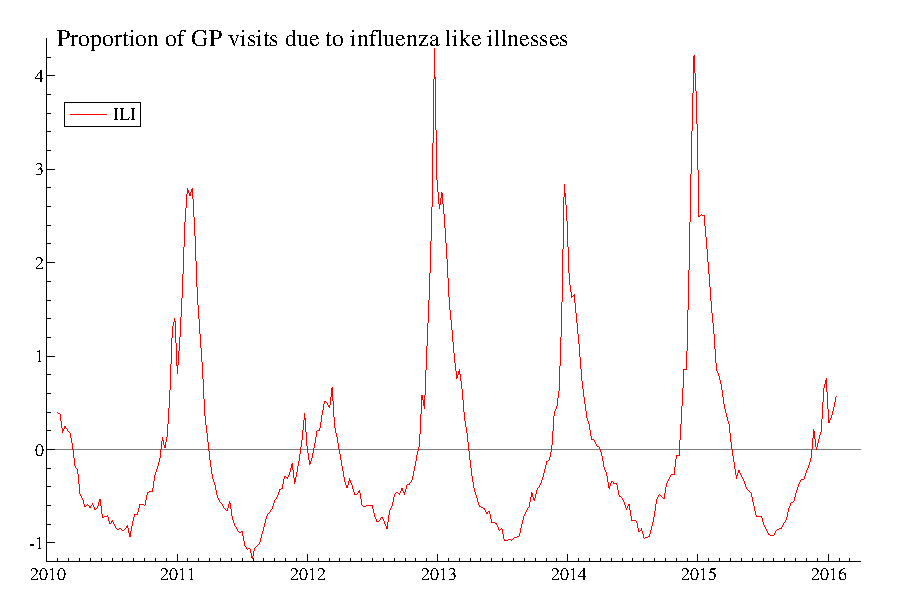
\includegraphics{ILIplot}
\caption{Proportion of GP visits due to influenza like illness}
\label{fig:ILIplot}
\end{figure}



\subsection{Google correlate data}

The search terms which are most correlated with ILI, called the correlates, as well as their first lags, are included in the GUM. To find these correlates, the weekly ILI time series was entered into the Google Correlate application. The sample entered into Google Correlate was different depending on the model, which will be explained in more detail below. Conveniently, like ILI, Google Correlate measures weeks from Sunday-Saturday. Google Correlate produced a list of the 100 search queries which were most correlated with ILI for the given sample, and provided the de-meaned search volume for those 100 search queries as weekly time series. The search volume for a particular query is the proportion of total search queries throughout a given week which were for that query. As a practical matter, Google Correlate data is available to the public with lag of several weeks. Acknowledging, however, that Google search query data is collected in real time, and in theory would be available for nowcasts, the nowcasting done here assumes that real time data is available. This approach is line with what was done with the original Google Flu Trends tool as well, making the results here comparable. 

\section{Nowcasting with Autometrics, Lasso and BSTS}

Nowcasting here is evaluated both using in-sample and out-of-sample results. Implementation of in-sample and out-of-sample models is relatively straightforward, as will be shown, using Autometrics and Lasso. As likely became apparent when the algorithms were described, BSTS is a much more complicated algorithm. Its main purpose, however, is nowcasting and there are features built into the BSTS R package which allow this to be done very easily. At a very basic level, nowcasts are made by drawing from the derived posterior distribution, and taking the mean across these MCMC simulations.  BSTS's reliance on Kalman filtering and smoothing, however, means that it is not (at this point) capable of producing "out-of-sample" nowcasts using this technique. Therefore, only in-sample nowcasting results are reported for BSTS. (Note: Scott Steve and I are in correspondence over this - hoping to have more clarification). 

\subsection{In-sample Nowcasting}
The in-sample nowcasting for Autometrics and Lasso used the entire sample period to estimate a model. The fitted values from this model are the nowcasts. The sample period was from week 5, 2010 to week 4, 2016 (The week beginning January 31 2010 to the week beginning on January 24 2016).

First, the GUM was identified. The GUM included any variables potentially relevant for modeling $ILI$. A quick glance at the graph of $ILI$ in Figure \ref{fig:ILIplot} indicates it is likely following an auto regressive process. $ILI$ peaks in the winter around Christmas and is at its lowest in the summer, indicating that seasonality is important. Therefore, lags 2-53 of $ILI$ were included in the GUM. Admittedly, this is not perfect as the number of weeks in a year varies and, for example, Christmas which likely is relevant to $ILI$ can fall in a different weeks. Other potential regressors included the 100 correlates, and their first lags.  Let $x_{1,t}, x_{2,t},...,x_{100,t}$ denote the search volumes of the top 100 correlates. These, their lags, and the lagged $ILI_{t}$ formed the GUM:

$$ILI_{t}= \alpha + \sum_{i=2}^{53}\gamma_{i}ILI_{t-i}+ \sum_{i=0}^{1}\sum_{j=1}^{100}\beta_{j,i}x_{j,t}+u_{t}$$

Next, the automatic model selection algorithms were applied to the above GUM. Autometrics and Lasso simply return a selected model and the fitted values. BSTS works in a slightly different way (it as a Bayesian algorithm after all), and has a built in predictor which simulates draws across the calculated posterior distributions for each $t$. Fitted values were found by taking the mean across these draws. Figure \ref{fig:InSample} graphs the fitted values against the de-meaned ILI values for each of the algorithms. The mean squared errors in Table \ref{MSEinsample} provide a clearer picture of how the various algorithms compare.   


\begin{landscape}
\begin{figure}
\centering
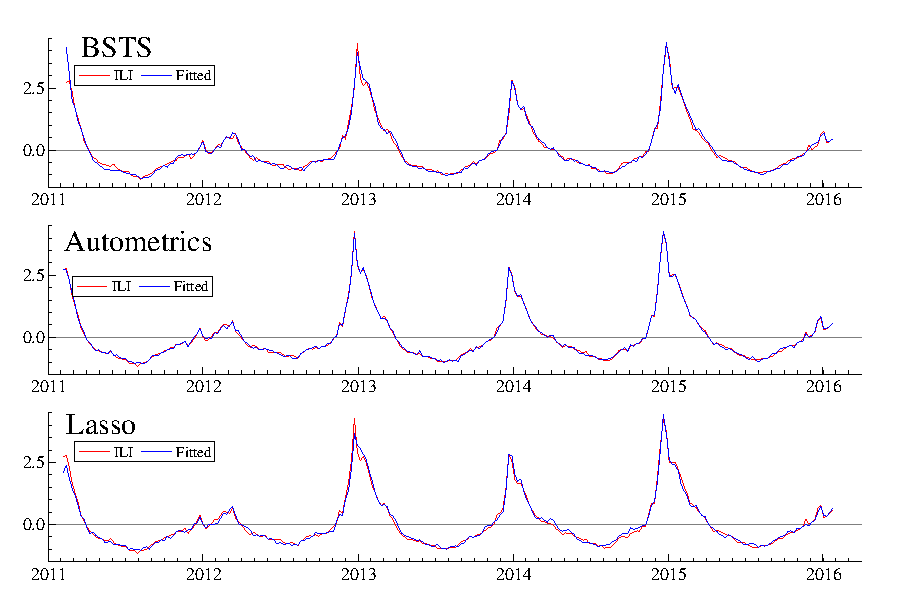
\includegraphics[scale=1.5]{All3plots}
\caption{In-sample nowcasts}
\label{fig:InSample}
\end{figure}
\end{landscape}




\begin{table}
\centering
\begin{tabular}{rr}
 & \textbf{MSE} \\
\textbf{Autometrics} & 0.003 \\
\textbf{Lasso} & 0.016\\
\textbf{BSTS} & 0.012  \\
    \end{tabular}%
      \caption{MSEs from in-sample nowcasting}
  \label{MSEinsample}%
\end{table}%

The table and graphs show that while all three algorithms are reasonably effective and nowcast with a high degree of accuracy, Autometrics does particularly well. More detailed output from running each of the models is provided in the Appendix (necessary?).

\subsection{Out-of-sample nowcasting}

In-sample nowcasting or forecasting where the GUM is the starting point obviously has the potential to be very accurate; the example of the extreme case of using OLS when $T=N$, and the fitted values exactly correspond to the true values comes to mind. Thus it is important to consider how nowcasts perform out-of sample. That is, how accurate a nowcast for time $t$ is, if the model relies only on information available up until time $t$. To take on this sort of approach in automatic model selection, there are several decisions that need to be made. It must be decided whether the algorithm should be applied and a new model selected each time a new observation is available. Another question is whether a rolling  or recursive forecast is more appropriate. An issue specific to using Google Correlates is whether a new set of correlates should be found each time an observation is added. 

To find out-of-sample nowcasts for ILI, the recursive nowcasting (or equivalently an expanding window) approach was used. The entire sample period went from Week 5, 2010 to Week 4, 2016 (the week beginning January 31 2010 to the week beginning on January 24 2016). The holdout period went from Week 5, 2015 to Week 4, 2016 (the week beginning February 01, 2015 to the week beginning January 24, 2016). Nowcasts were made for each of the 52 weeks in the holdout period, with a new model being selected, and a new fitted value being found for each of the 52 nowcasts. Google correlates were found using the ILI data from Week 5, 2010 to Week 4, 2015 and thus the correlates in the GUM remained the same in each nowcast model. Thus for each $t$ for a which a nowcast produced, the algorithms commenced from the following GUM:

$$ILI_{t}= \alpha + \sum_{i=2}^{53}\gamma_{i}ILI_{t-i}+ \sum_{i=0}^{1}\sum_{j=1}^{100}\beta_{j,i}x_{j,t}+u_{t}$$

The model selected at time $t$ was used to find the fitted value, or nowcast for time $t$. The fitted values and true ILI are graphed for Autometrics and Lasso in Figure \ref{fig:OutofSample}. The nowcast MSE are in Table \ref{MSEoutofsample}. Both Autometrics and Lasso perform well, with Lasso achieving a slightly smaller MSE than Autometrics. 

\begin{figure}
\centering
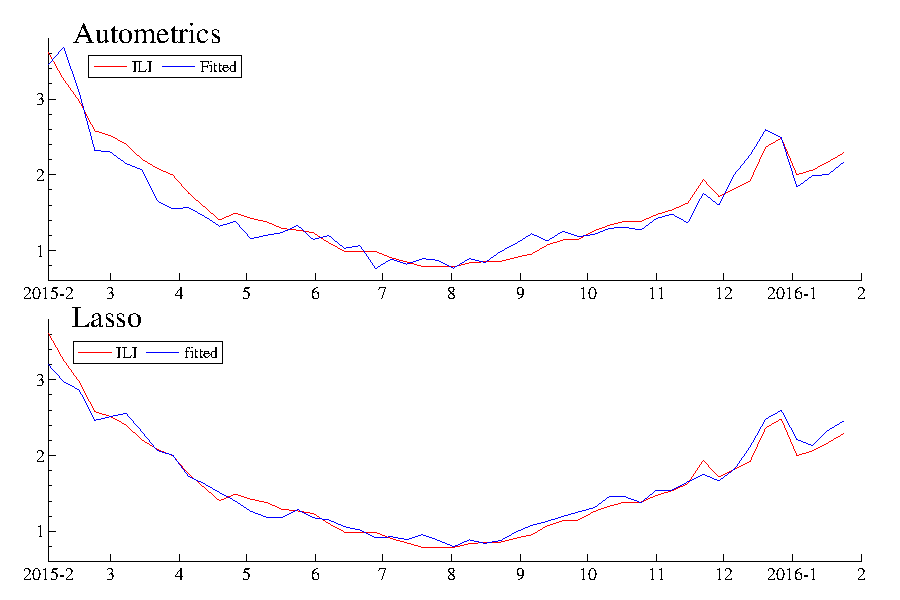
\includegraphics{LassoAuto}
\caption{Out-of-sample Nowcasts}
\label{fig:OutofSample}
\end{figure}

\begin{table}
\centering
\begin{tabular}{rr}
 & \textbf{MSE} \\
\textbf{Autometrics} & 0.032 \\
\textbf{Lasso} & 0.014 \\

    \end{tabular}%
      \caption{MSEs from out-of-sample nowcasting}
  \label{MSEoutofsample}%
\end{table}%

\subsection{Original Google Flu Trends Estimates}

Since its inception in 2008, the Google Flu Trends model has been updated three times, most recently in 2014. While Google has never released the algorithm it used to compute its ILI estimates, the estimates themselves are available. It has also released the estimates that the revised models produce when applied to historical data. An interesting exercise is then to see how these estimates compare to the estimates produced using the algorithms studied here. 

Figure \ref{fig:2014GFT} graphs the estimates produced by Google's 2014 model. Note that it is not clear whether these are in-sample or out-of-sample nowcasts. The nowcast MSE is 0.021, which is much larger then Autometrics in-sample MSE and smaller than both the in-sample and out-of-sample Lasso MSE.  


\begin{figure}
\centering
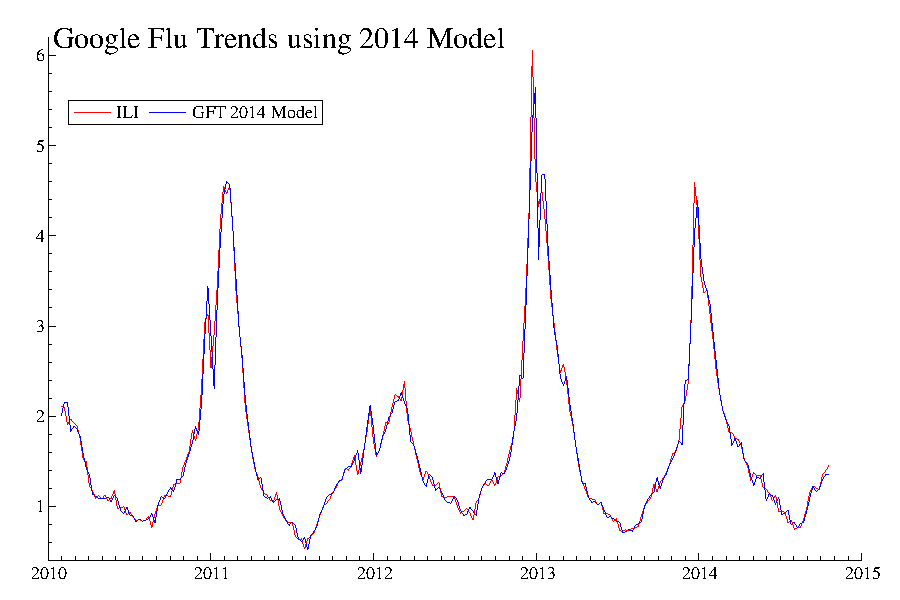
\includegraphics{GFT2014}
\caption{Nowcasts for 2010-2015 using Google's 2014 model}
\label{fig:2014GFT}
\end{figure}

\section{Nowcasting take-aways}

As this chapter shows, nowcasting is an interesting, relevant and useful application of automatic model selection. Depending on the complexity of the algorithm, it can also be employed very easily. As the way that economic data is collected begins to change, and as it starts to become available in real-time automatic model selection for nowcasting could become a very useful tool for economist, statistical agencies and policy makers alike.  










\chapter{Meeting notes}

\section{Meeting 1: March 27th, 2015}
\textbf{What was discussed:}
\begin{itemize}
\item Big data has become a big topic in computer science and also in economics
\item Economics and in particular macroeconomics, could stand to benefit from the increasingly available amount of data
\item The difficult and still relatively new aspect of big data is how to analyse it (particularly for economic purposes)
\item In particular for economists who are often interested in casual relationships, big data involves many, many (hundreds, thousands) of variables and thus standard
econometric techniques do not necessarily apply
\item Machine learning is increasingly becoming an important tool in the economist (and
specifically econometrician) toolkit 
\item There are differing ideas on how to analyse big data - i.e. Autometrics vs. other ML techniques !
\item There are a number of different machine learning techniques which are beginning to be noticed by economists. Namely, Hal Varian is a big proponent of machine learning (neural nets, pruning trees, etc.. ?Big Data: New Tricks for Econometrics? paper)
\item Varian/Google do a lot with search query data and look at how it can be used as a predictor (i.e. for the flu) although there are varying opinions on how valid/accurate these techniques actually are !
\item Castle, Hendry, and Doornik have a different idea as to how to deal with big data, which is embodied in Autometrics
\item The Autometrics algorithm is an automatic model selection algorithm, which essentially searches through data and returns the model which best fits the data
\item It uses a variety of techniques and allows for different combinations of data to return the best possible model
\item Autometrics uses a technique which allows you to have N>T candidate variables 
\item Autometrics is different from other machine learning techniques - much debate over which is better
\item It would be useful to test Autometrics against other machine learning techniques (particularly those that Hal Varian likes)
\item Felix Pretis has a ?big data? data set which Autometrics could analyse and could
also be analysed via other machine learning algorithms 
\item It would be interesting to evaluate, one way or another, which algorithm is ?better?
\item Perhaps could compare the different approaches by comparing respective nowcasts
\end{itemize}

\textbf{Thesis Idea/General Outline:}
\begin{itemize}
\item My thesis will examine the Autometrics algorithm in comparison to other ML algorithms
\item Will most likely use Felix Pretis?s data set which will require serious manipulation/ cleaning to become useable, but should be sufficient to analyse via the different techniques
\item The aim will be to use both (or multiple) techniques to analyse the data set and produce nowcasts/forecasts/predictions (or some other measure which will allow for comparison between the different techniques)
\item Possible ML learning techniques include the ones outlined in Varian?s paper
\item Would be great to gain access to ML algorithms directly from companies in Silicon
Valley (i.e. an old colleague who works as for a data analysis company) 
\item This colleague who is very knowledgable on ML has agreed to at least be a
resource and will help me with the ML side of things (even if he can?t give up hisalgorithms)
\item There are also lots of open source algorithms available online which will likely prove
very useful 
\end{itemize}

\textbf{Preliminaries/First Steps:}
\begin{itemize}
\item Solid understanding of how Autometrics works, specifically how it deals with structural breaks, small effects, how it can be used for nowcasting
\item Understanding of other ML techniques and how they differ from Autometrics!
\item Coding skills required to clean the data
\item Actually cleaning the data so that it is in an appropriate format (i.e. so that we can
test out Autometrics and other algorithms) 
\end{itemize}

\textbf{Timeline}:
\begin{itemize}
\item I would like to take the summer to do a fair amount of reading to gain a comprehensive understanding of autometrics and other ML algorithms 
\item I think the summer would also be a good time to start cleaning and getting a feel for the data so that I can begin my analysis in Michaelmas next year!
\item Basically, I would like to use the summer to both gain a thorough amount of background knowledge, as well as do most of the ?dirty work? which will be required to undertake this research !
\end{itemize}


\section{Meeting 2: October 22nd, 2015}
\textbf{Data Update Generated Data}
\begin{itemize}
\item Ox code is ready and running and able to be adjusted for multiple scenarios: i.e. structural breaks, different numbers of regressors
\item Based on code from Strucutural Break paper
\item This data will be main focus of thesis and what I will focus on first
\end{itemize}
\textbf{Google Flu Data}
\begin{itemize}
\item Downloaded from Google Correlate application
\item While Google has never explicitly provided the algorithm they used for Google Flu Trends, the Nature paper describes the method used
\item From this paper, the data required are search volumes of the search queries most correlated with the Influenza Like Illness statistic published bythe Centre for Disease Control in America
\item This data is downloaded and ready to use
\end {itemize}

\textbf{Alogirthms update}
\begin{itemize}
\item Three definite algorithms to be used for sure: Autometrics, Lasso, Bayesian Structural Time Series
\item Autometrics: running through OxMetrics
\item Lasso: running through R
\item Bayesian Structural Time Series: running through R
\item Two other possibilities: Bayesian technique from Nature paper and possibly neural networks for time series
\item Bayesian techniques from Nature paper by Ghahramani is likely quite easy to include as another method
\item Jennie has a contact who is working on neural networks for time series: will provide his information
\end{itemize}

\textbf{Current plan}
\begin{itemize}
\item begin analysis: starting with generated data and Autometrics
\item Goal: to have analysis + first draft of write up of generated data completed by end of Christmas break
\end{itemize}

\section{Meeting 3: November 5th, 2015}
\begin{itemize}
\item General discussion of how to consolidate everything I've been doing
\item Decided on formulation of several different DGP's to simulate
\begin{itemize}
\item Number of observations constant across simulations at T=100
\item With respect to number of regressors: one case with N=80 (N\textless T), one case with N=120 (N\textgreater T)
\item Number of relevant regressors can remain fixed in each experiment at $n=5$
\item Value of $\beta$ coefficients: variations should include:
\begin {itemize}
\item $\beta_{1}=...=\beta_{5}=0.2$
\item $\beta_{1}=...=\beta_{5}=0.6$
\item $\beta_{1}=0.2, \beta_{2}=0.3, \beta_{3}=0.4, \beta_{4}=0.5, \beta_{6}=0.6$
\end{itemize}
\item Significance level should be no greater than 0.01
\item Should consider cases with both orthogonal and correlated regressors
\item Also should consider structural breaks: but leave this for now
\end{itemize}
\item For next week: consolidate everything that I've done + results
\end{itemize}

\section{Meeting 4: November 19th, 2015}
\begin{itemize}
\item Discussion of results of Autometrics and LASSO - in simulations Autometrics performs far better than LASSO and gauge and potency are approximately  what theory would expect them to be
\item Discussion over what to set lambda to in LASSO - consensus that it really doesn't matter because it won't drastically change results and most people don't know enough about it anyways to make it worth worrying about
\item Apparently LASSO can be run in Ox - can likely find code from online textbook - will look into this
\item Up next: get BTST up and running + finish up LASSO on initial experiments
\item David mentioned another data set by a guy at Oxford - Steve Bro...?? This could potentially be an excellent economic application of what I'm working on 
\item Results from Autometrics and LASSO are at the end of this document
\end {itemize}


\section{Meeting 4: November 19th, 2015}
\begin{itemize}
\item Discussion of results of Autometrics and LASSO - in simulations Autometrics performs far better than LASSO and gauge and potency are approximately  what theory would expect them to be
\item Discussion over what to set lambda to in LASSO - consensus that it really doesn't matter because it won't drastically change results and most people don't know enough about it anyways to make it worth worrying about
\item Apparently LASSO can be run in Ox - can likely find code from online textbook - will look into this
\item Up next: get BTST up and running + finish up LASSO on initial experiments
\item David mentioned another data set by a guy at Oxford - Steve Bro...?? This could potentially be an excellent economic application of what I'm working on 
\item Results from Autometrics and LASSO are at the end of this document
\end {itemize}


\section{Meeting 7: February 4th, 2016}
\begin{itemize}
\item Discussion of results in latest draft included a number of corrections and suggestions.
 
\item In the tables for retention rates, gauge and potency:
\begin{itemize}
\item Non centralities are being calculated incorrectly: I was using T instead of N and thus getting different results for $N<T$ and $N>T$. We went over the formula and this will be corrected.
\item Should possibly change the $\beta$ coefficients so that the non-centralities are more easily understood - i.e. 2, 3, 4,...: there are several ways to do this. The $\rho$ used to generated the regressors (in $x_{t} = \rho x_{t-1} + v_{t}$) makes things slightly more complicated - but still something to consider. Non-centralities of 2, 2.5, 3... would be more inline with what is published in the existing literature.
\item Theoretical retention probabilities should be included in the tables for each non-centrality .
\item Need to explicit outline how selection from LDGP is being done (i.e. explain one-cut selection).
\item Also need to calculate theoretical retention probabilities with selection from LDGP
\item We discussed that selection from the LDGP when the regressors are non-orthogonal is not a useful benchmark. Instead I will include the results of selection from LDGP using Autometrics, Lasso and BSTS (without changing the settings in BSTS).
\end{itemize}
\item I need to include a discussion on the costs of inference and costs of search across the methods.
\item A new plot which shows potency against gauge would be a nice way to present the results: suspect this would result in clusters for each of the three algorithms. 
\item Early results from non-orthogonal case are very strange: 

\begin{itemize}
\item With alternating signs ($\beta_{1}=-0.2$, $\beta_{2}=0.3$, $\beta_{3}=-0.4$, $\beta_{4}=0.5$, $\beta_{5}=-0.6$) and high correlation across the relevant regressors (covariance between regressors is $\rho=0.99$)  both Lasso and Autometrics are doing the opposite of what we'd expect. The retention rate of $x_{1}$ (the variable with the smallest non-centrality) is far higher than any of the other variables - in fact, the retention rate in general is decreasing as the non-centrality is increasing. 
\item In BSTS, the retention rate of variables with negative coefficients is higher than those with positive coefficients. 
\item We were all rather confused by these results - it could be something funny going on in the Autometrics and Lasso programs themselves. I will investigate some more. David - perhaps you have an explanation?
\end{itemize}
\item Will also run some simulations where all N variables are correlated.
\item Discussion of MSE tables:
\begin{itemize}
\item Will include a graph based on David's suggestion: Jennie suggested average RMSE for retained irrelevant variables across the different methods
\item The bench mark for MSEs should be the MSEs from the LDGP - will calculate and include this in the table.
\item While using bias correction is perhaps not necessary (if I did it for Autometrics, I could do something similar for Lasso - methods do exists and it wouldn't seem 'fair' to only do it for Autometrics) a discussion of bias correction should at least be included. This includes the direction of bias, what we expect the distribution of the MSEs to be as well as graphs illustrating this.  
\item Jennie suggested only including conditional MSE - the unconditional MSE aren't all that useful.
\end{itemize}
\item Should also start thinking about exactly which tables and graphs should be included in final document. An appendix would possibly be useful.
\item We also discussed that there are many, many simulations I could do in theory - but perhaps getting onto the empirical section would be useful. This could provide direction for other simulations which might be useful.  



\end {itemize}

\chapter{Results}










\end{document}  